\section{Resoconto attività di verifica}
\subsection{Verifica dei documenti}
\subsubsection{Indice di Gulpease}
L'Indice Gulpease è un indice di leggibilità di un testo tarato sulla lingua italiana. Rispetto ad altri ha il vantaggio di utilizzare la lunghezza delle parole in lettere anziché in sillabe, semplificandone il calcolo automatico.
I risultati sono compresi tra 0 e 100, dove il valore "100" indica la leggibilità più alta e "0" la leggibilità più bassa. In generale risulta che testi con un indice
\begin{itemize}
    \item inferiore a 80 sono difficili da leggere per chi ha la licenza elementare;
    \item inferiore a 60 sono difficili da leggere per chi ha la licenza media;
    \item inferiore a 40 sono difficili da leggere per chi ha un diploma superiore.
\end{itemize}

Di seguito vengono mostrati i risultati dell’indice di Gulpease per ogni documento redatto, escludendone la prima pagina, registro delle modifiche, l'indice e gli elenchi di figure e tabelle.

\renewcommand{\arraystretch}{1.8}
\begin{xltabular}{\textwidth} {
        >{\hsize=1.4\hsize\linewidth=\hsize}X
        >{\hsize=0.8\hsize\linewidth=\hsize}X
        >{\hsize=1\hsize\linewidth=\hsize}X
    }
    \rowcolorhead
    \textbf{\color{white}Documento} &
    \textbf{\color{white}Valore indice} &
    \textbf{\color{white}Esito}\\
    \hline
    \endfirsthead

    \hline
    \rowcolorhead
    \textbf{\color{white}Documento} &
    \textbf{\color{white}Valore indice} &
    \textbf{\color{white}Esito}\\
    \hline
    \endhead

    \endfoot

    \endlastfoot

    \textit{Analisi dei Requisiti v2.0.0}&
    67 &
    Superato
    \\ \hline

    \textit{Norme di Progetto v2.0.0}&
    72 &
    Superato
    \\ \hline

    \textit{Piano di Progetto v2.0.0}&
    67 &
    Superato
    \\ \hline

    \textit{Piano di Qualifica v2.0.0}&
    80 &
    Superato
    \\ \hline

    \textit{Specifica Tecnica v1.0.0}&
    70 &
    Superato
    \\ \hline

    \textit{Glossario v2.0.0}&
    69 &
    Superato
    \\ \hline

    \textit{Verbale 2022/10/24}&
    72 &
    Superato
    \\ \hline

    \textit{Verbale 2022/10/25}&
    73 &
    Superato
    \\ \hline

    \textit{Verbale 2022/10/26}&
    74 &
    Superato
    \\ \hline

    \textit{Verbale 2022/10/26}&
    70 &
    Superato
    \\ \hline

    \textit{Verbale 2022/10/28}&
    75 &
    Superato
    \\ \hline

    \textit{Verbale 2022/11/08}&
    75 &
    Superato
    \\ \hline

    \textit{Verbale 2022/11/12}&
    75 &
    Superato
    \\ \hline

    \textit{Verbale 2022/11/23}&
    74 &
    Superato
    \\ \hline

    \textit{Verbale 2022/12/14}&
    76 &
    Superato
    \\ \hline

    \textit{Verbale 2023/01/15}&
    74 &
    Superato
    \\ \hline

    \textit{Verbale 2023/01/20}&
    73 &
    Superato
    \\ \hline

    \textit{Verbale 2023/01/24}&
    76 &
    Superato
    \\ \hline

    \textit{Verbale 2023/02/19}&
    75 &
    Superato
    \\ \hline

    \textit{Verbale 2023/03/20}&
    78 &
    Superato
    \\ \hline

    \textit{Verbale 2023/03/25}&
    79 &
    Superato
    \\ \hline

    \textit{Verbale 2023/03/28}&
    85 &
    Superato
    \\ \hline

    \textit{Verbale 2023/03/30}&
    84 &
    Superato
    \\ \hline

    \textit{Verbale 2023/03/31}&
    80 &
    Superato
    \\ \hline

    \rowcolor{white}
    \caption{Risultati indice di Gulpease}
\end{xltabular}

\subsection{Verifica dei processi}

\subsubsection{Estimated at Completion}

\begin{figure}[H]
\centering
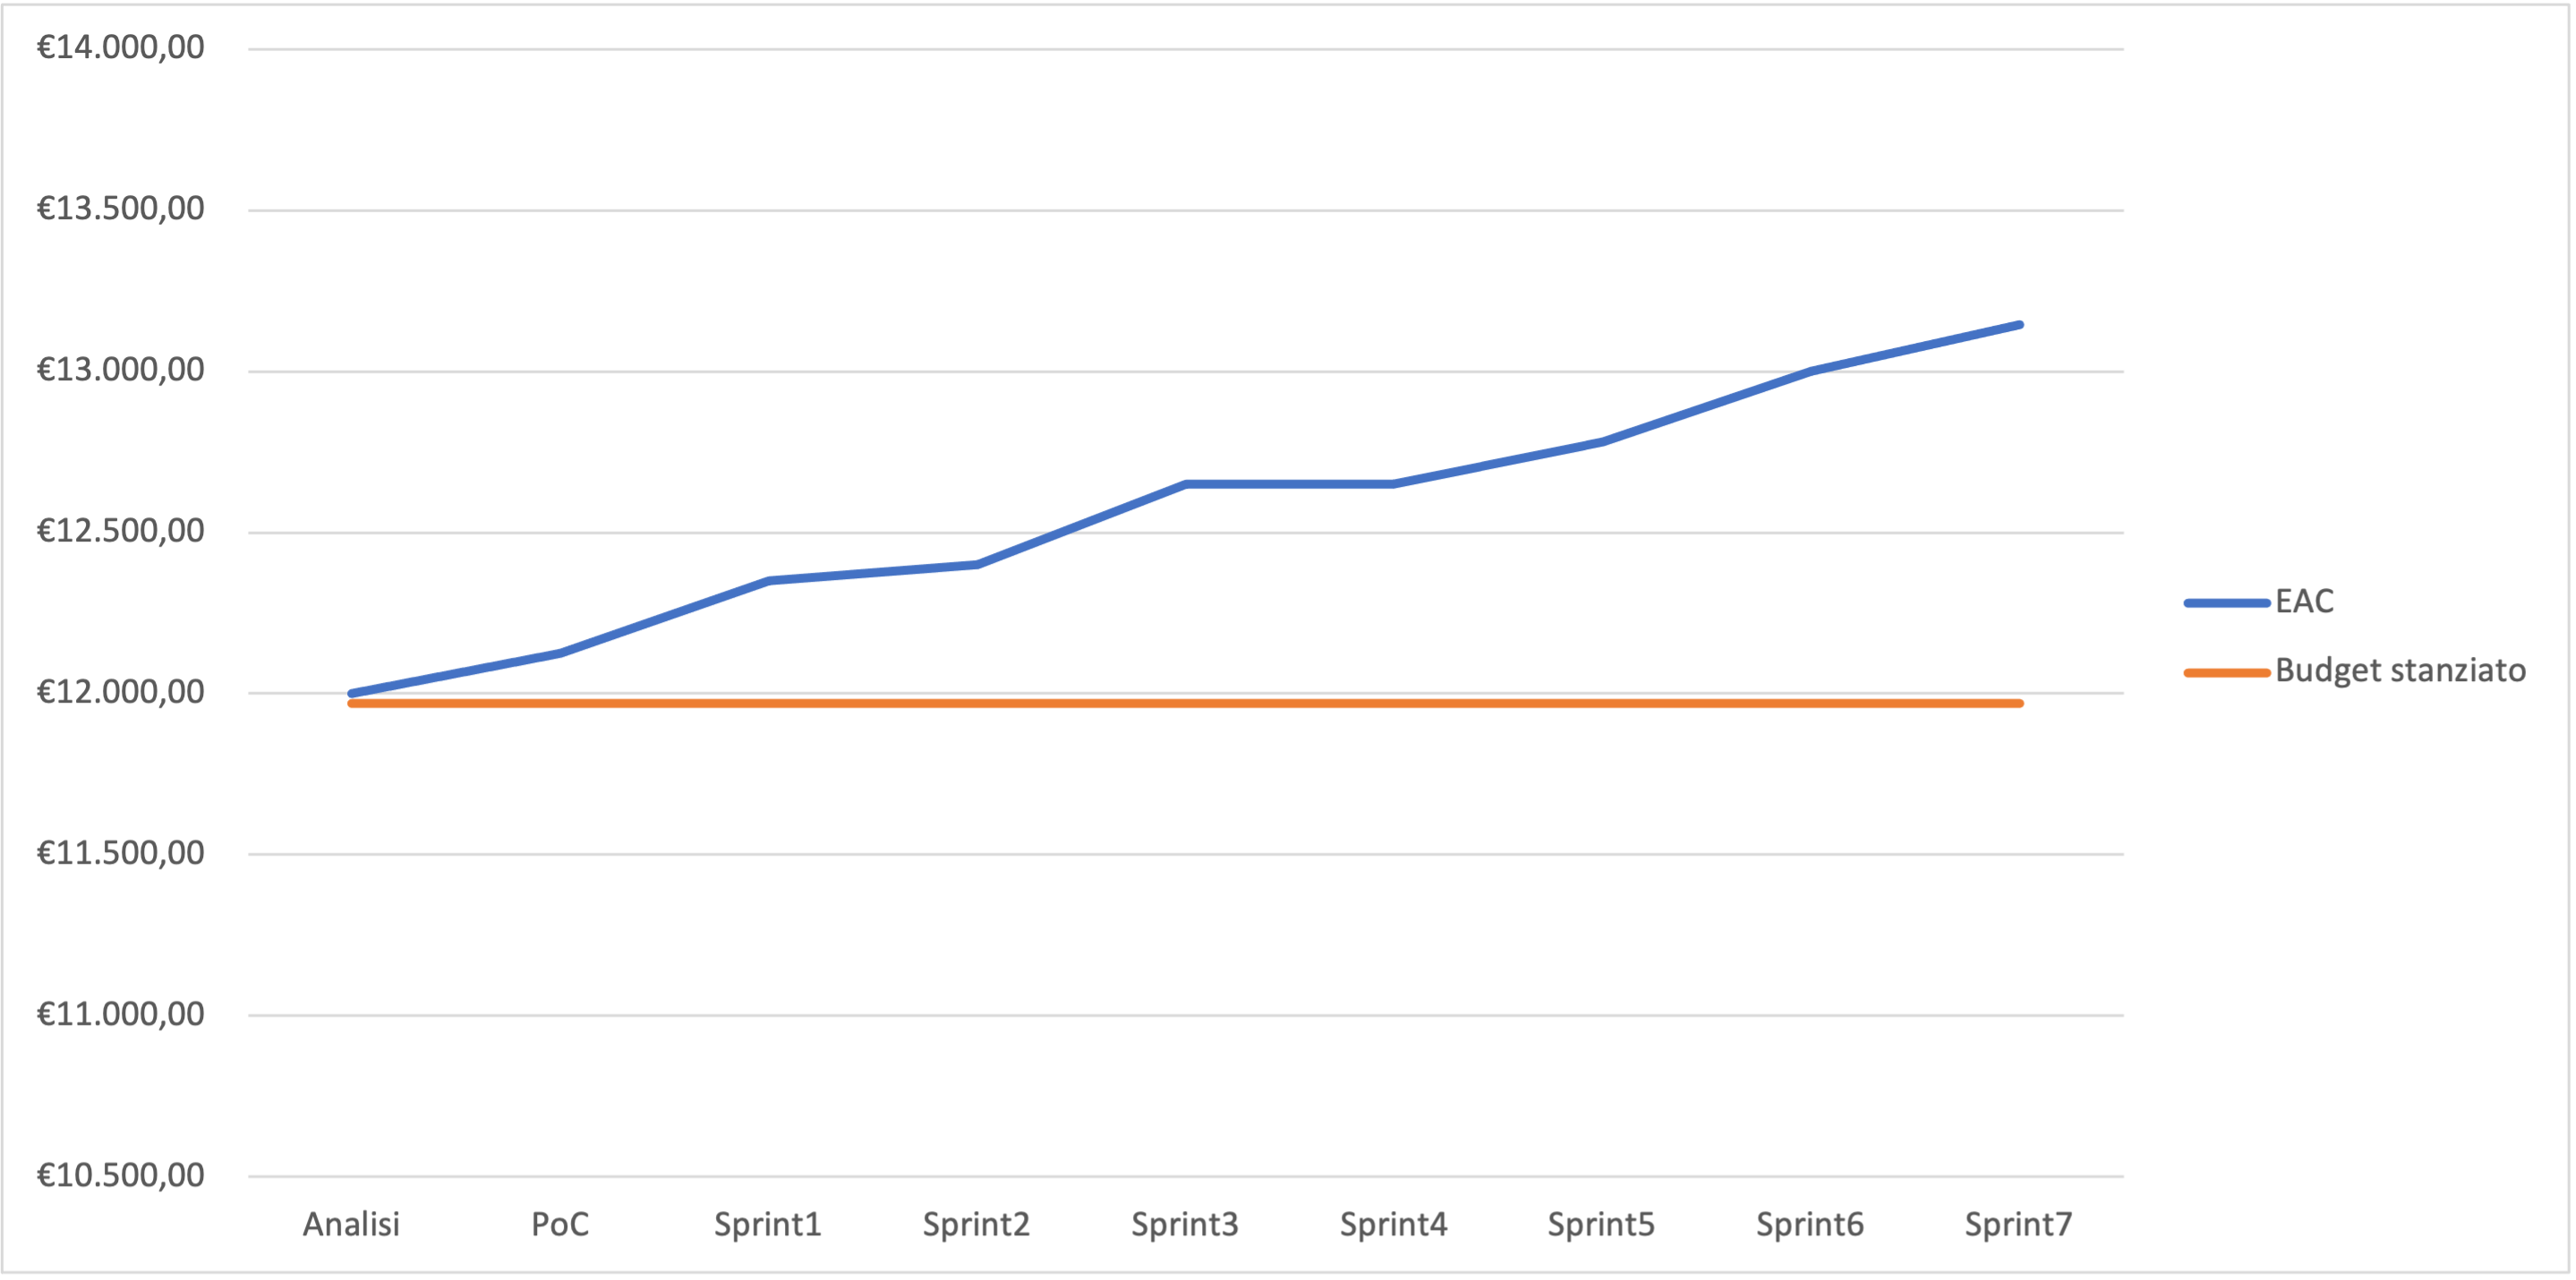
\includegraphics[width=1\textwidth]{src/img/EAC.png}
\caption{Grafico EAC}
\end{figure}

\subsubsection{Earned Value e Planned Value}

\begin{figure}[H]
\centering
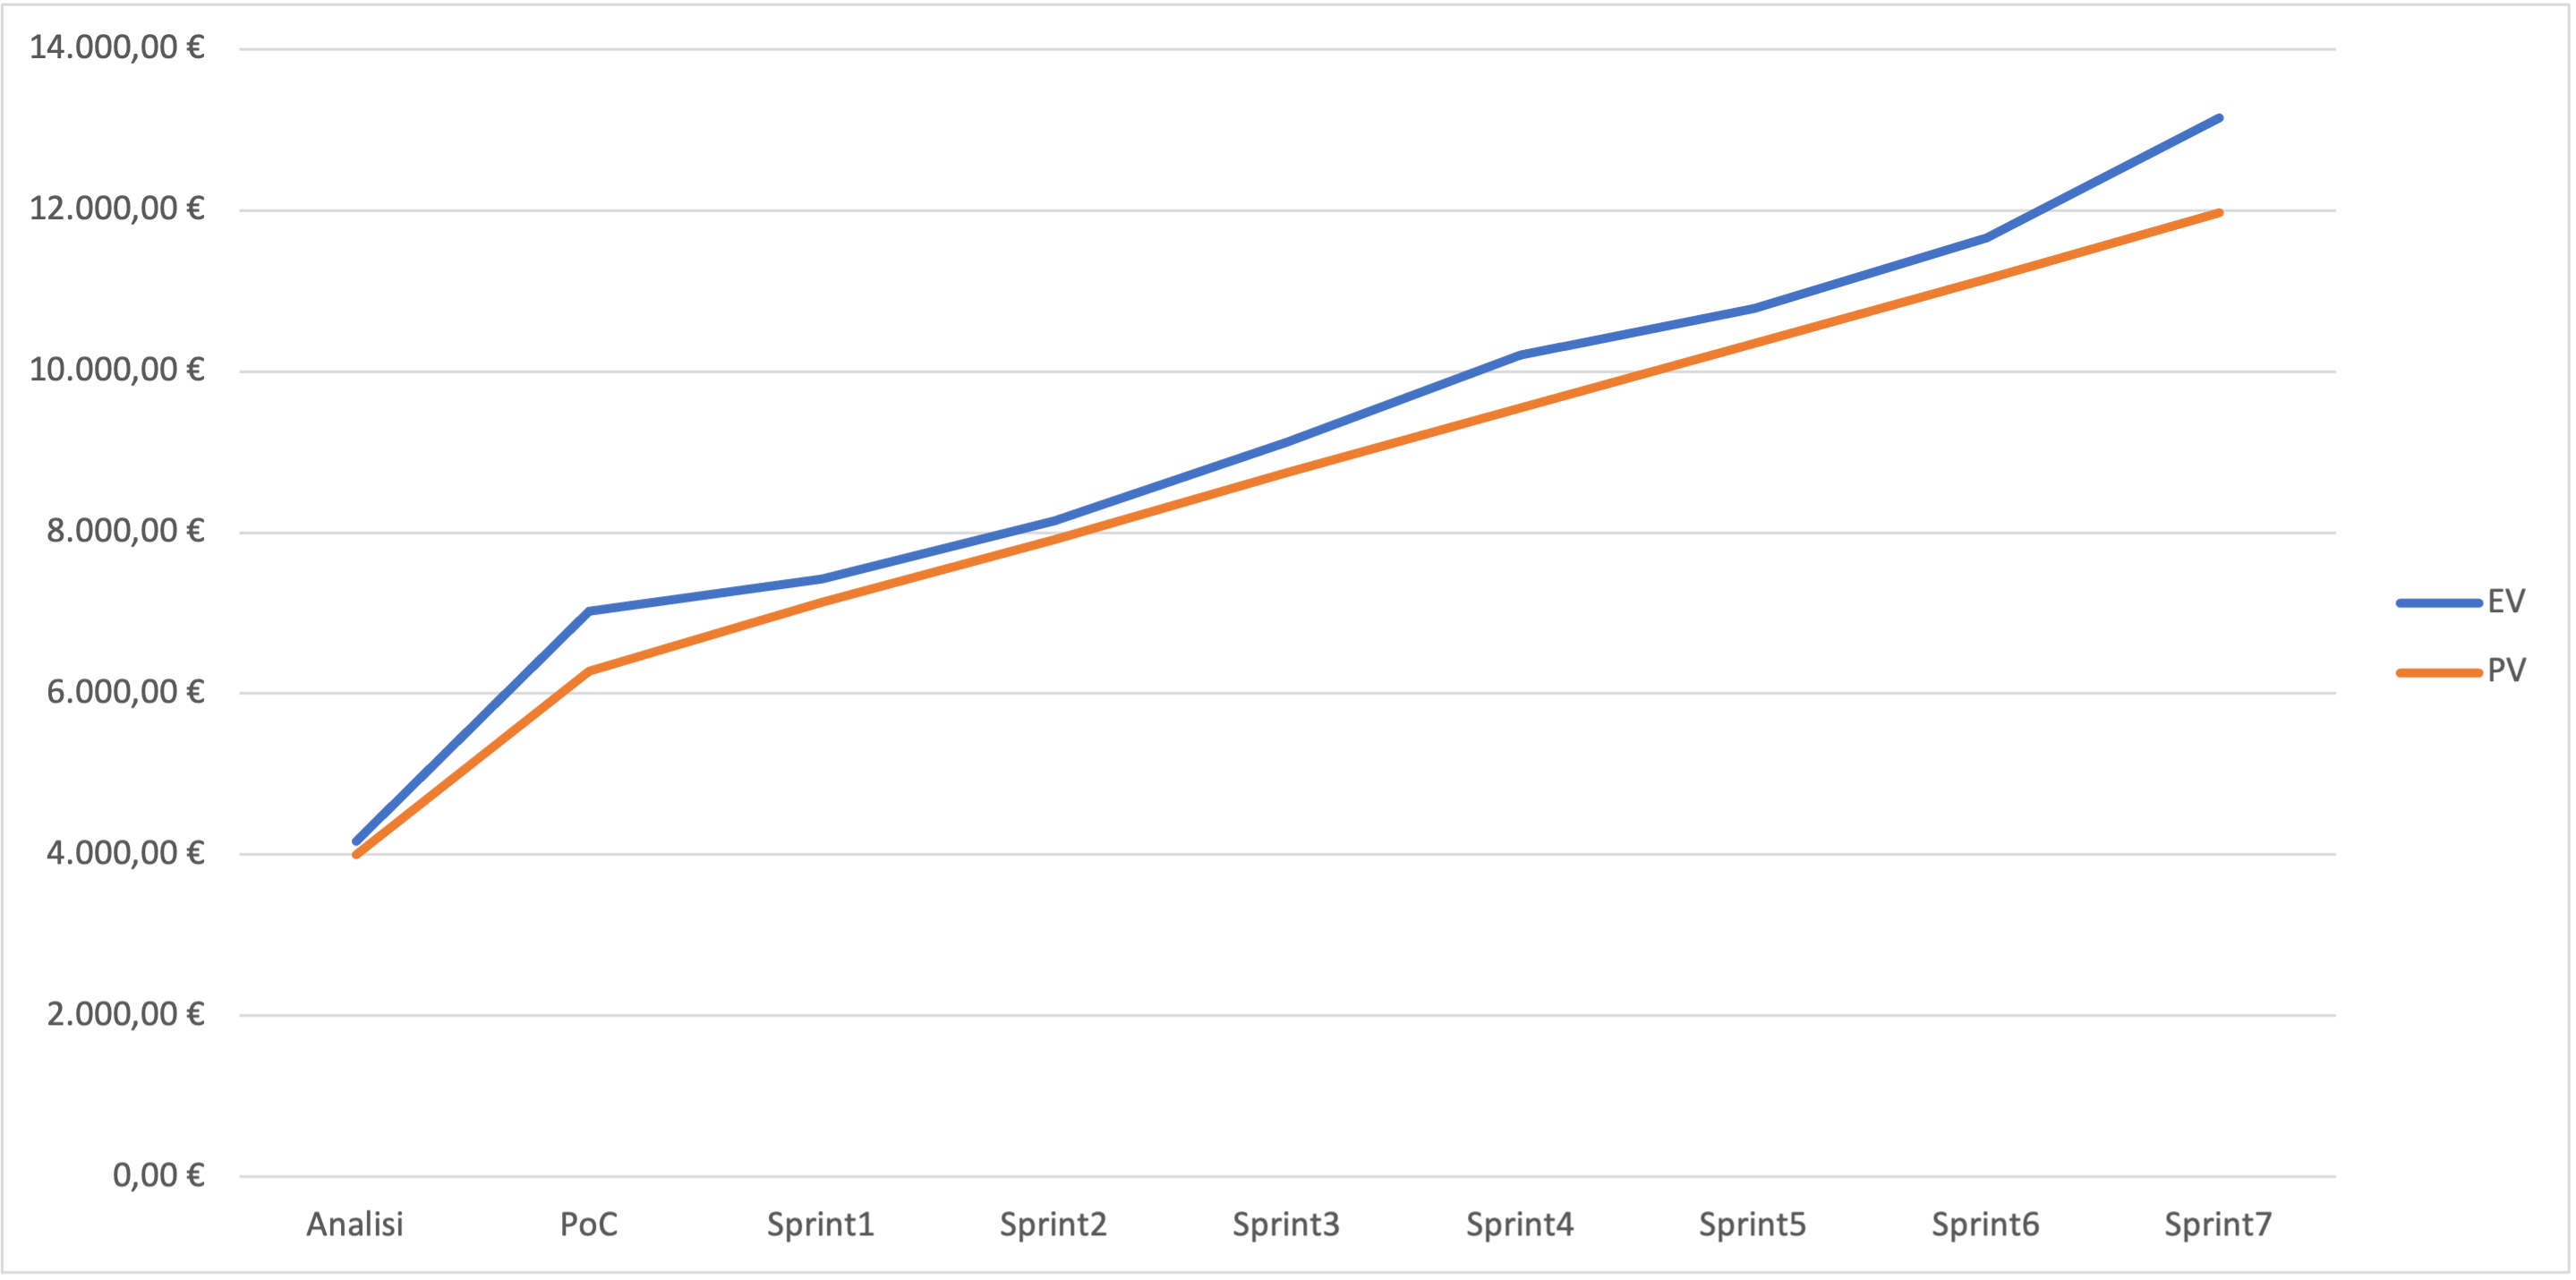
\includegraphics[width=1\textwidth]{src/img/EVPV.png}
\caption{Grafico EV, PV}
\end{figure}

\subsubsection{Actual Cost e Estimate To Complete}
\begin{figure}[H]
\centering
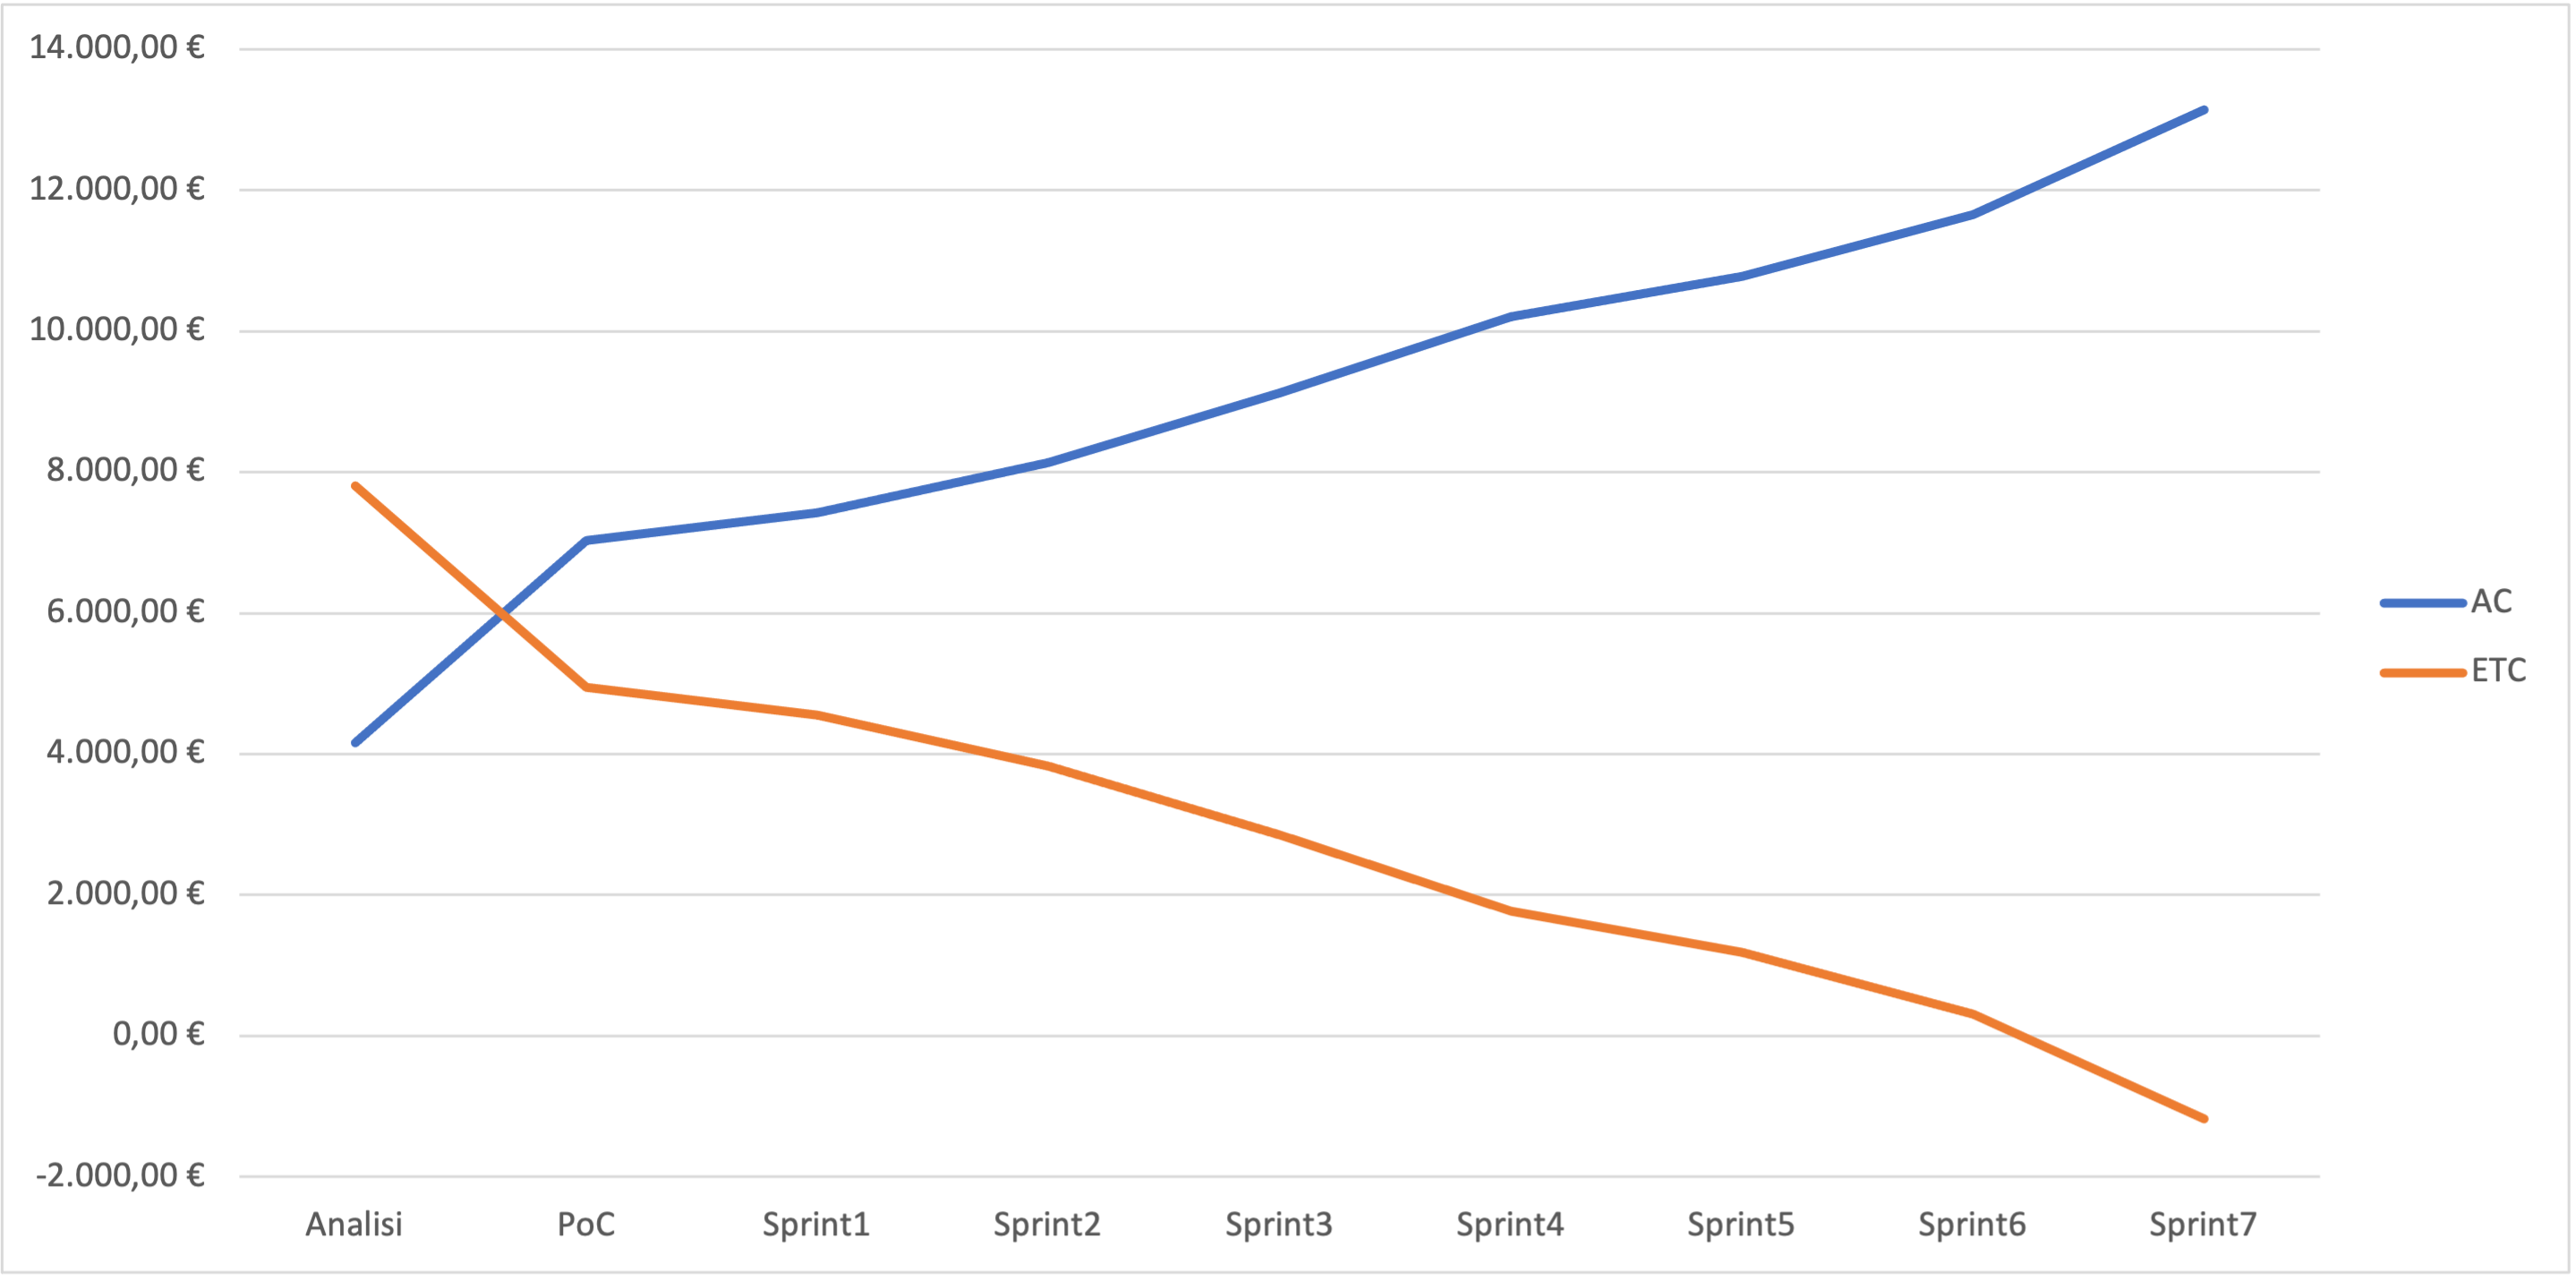
\includegraphics[width=1\textwidth]{src/img/ACETC.png}
\caption{Grafico AC, ETC}
\end{figure}

\subsubsection{Schedule Variance e Cost Variance}
\begin{figure}[H]
\centering
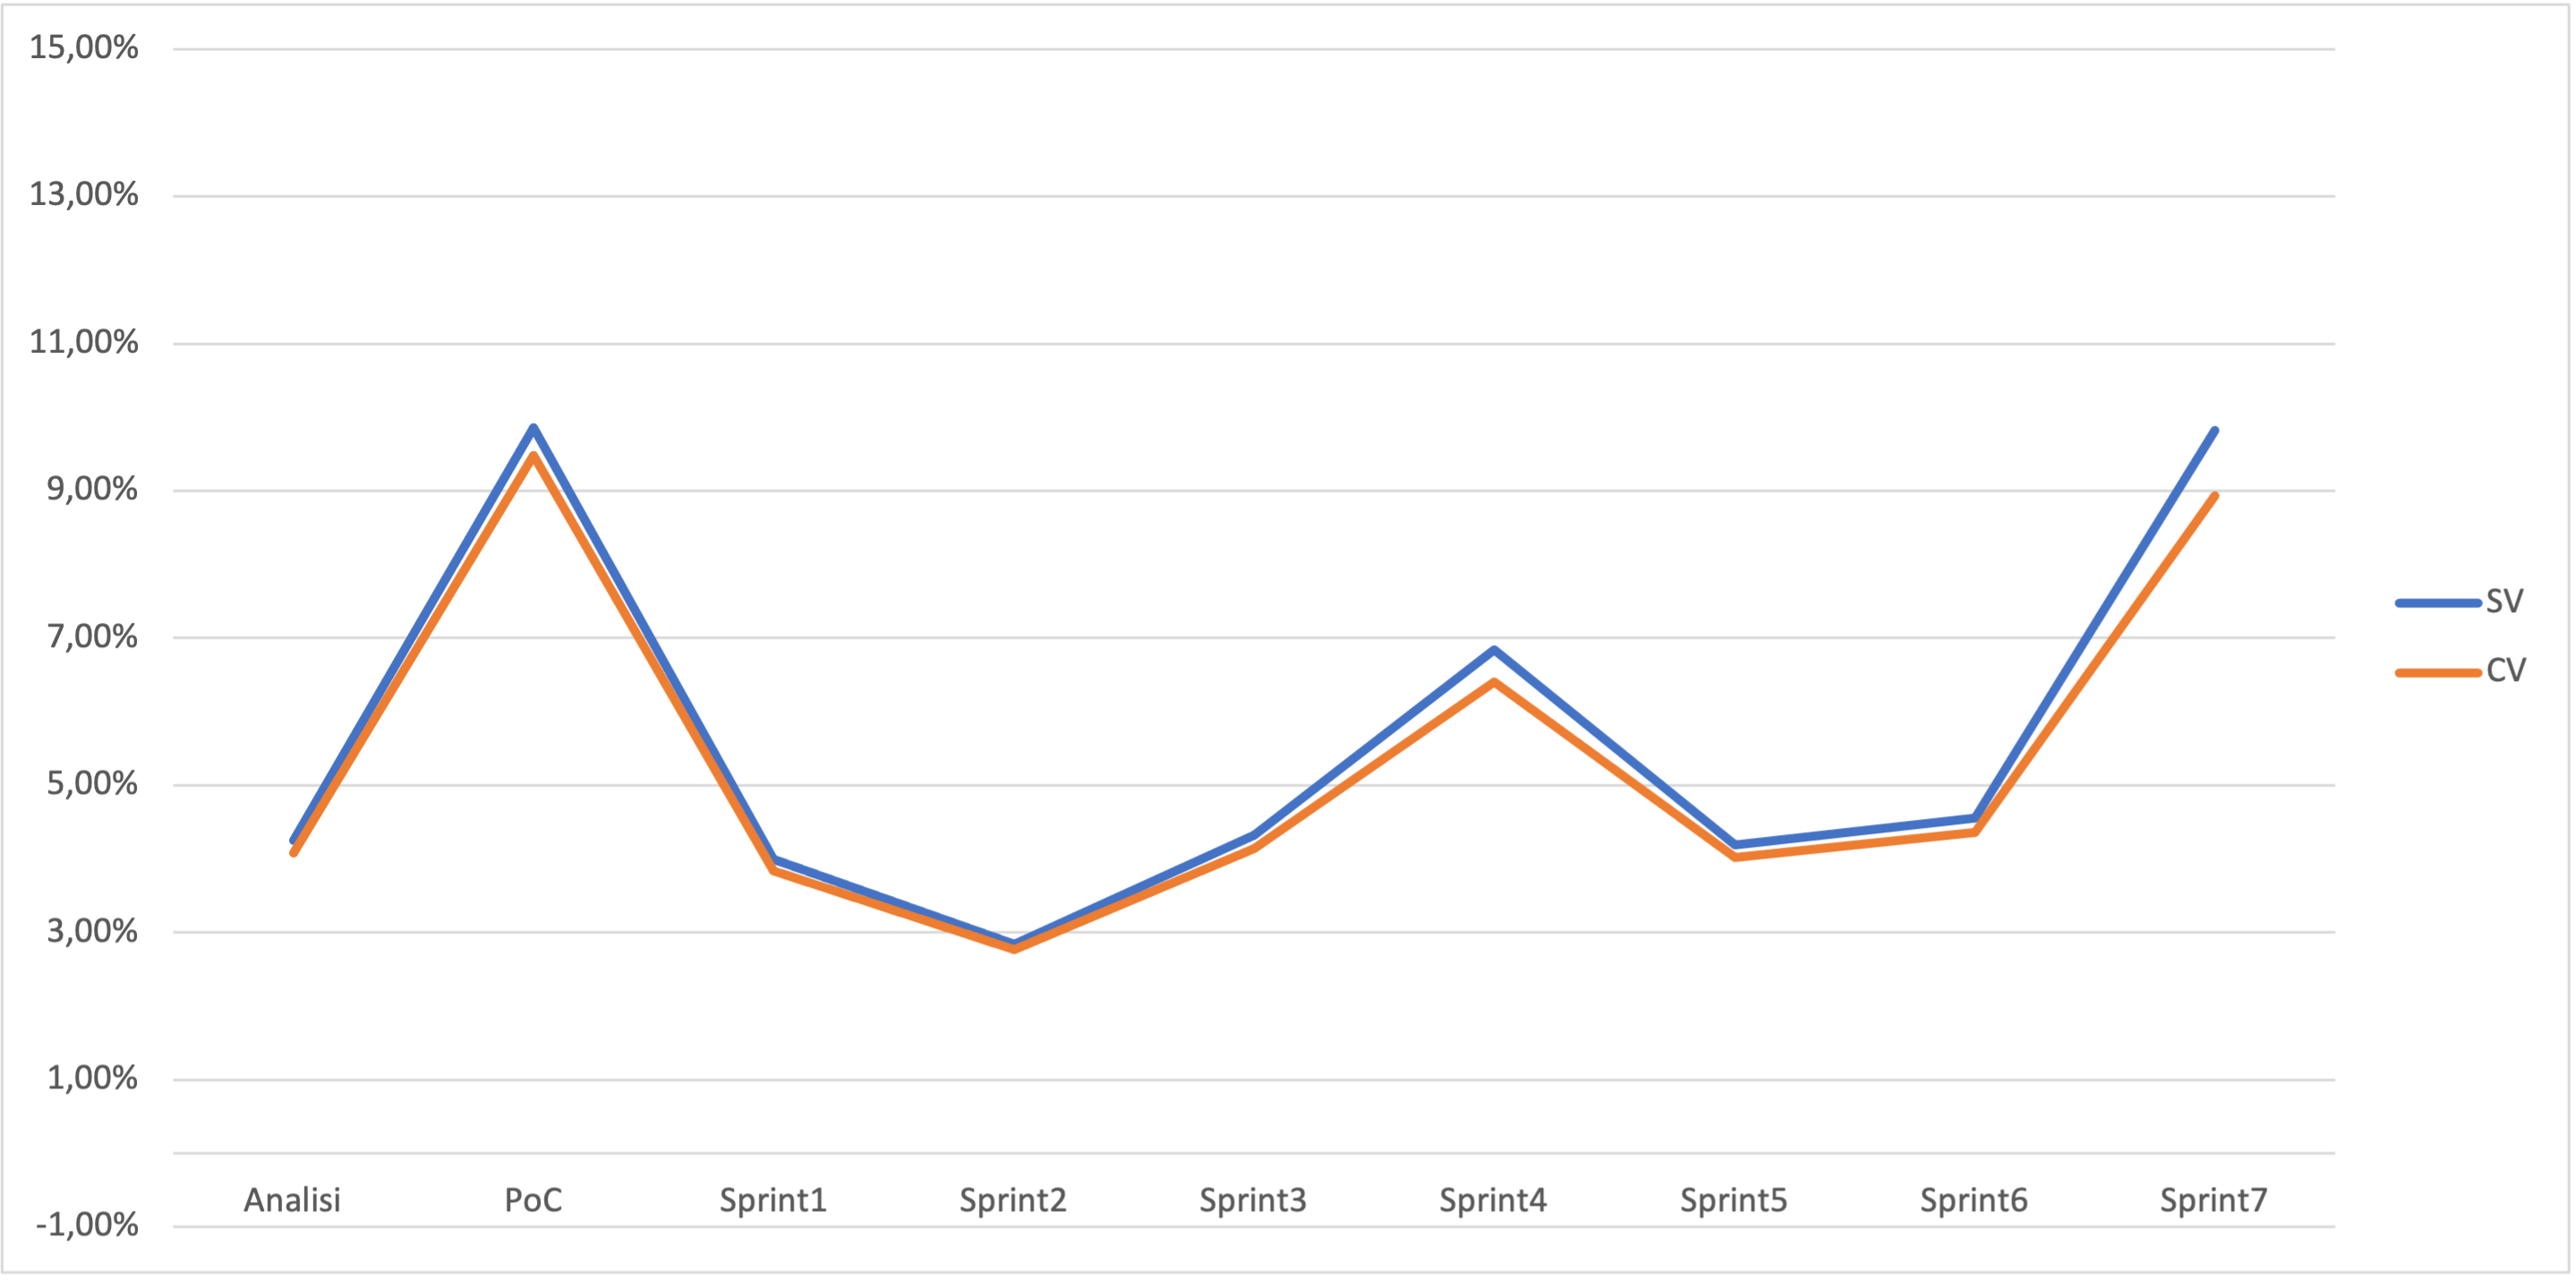
\includegraphics[width=1\textwidth]{src/img/SVCV.png}
\caption{Grafico SV, CV}
\end{figure}

\subsubsection{Requirements Stability Index}
\begin{figure}[H]
\centering
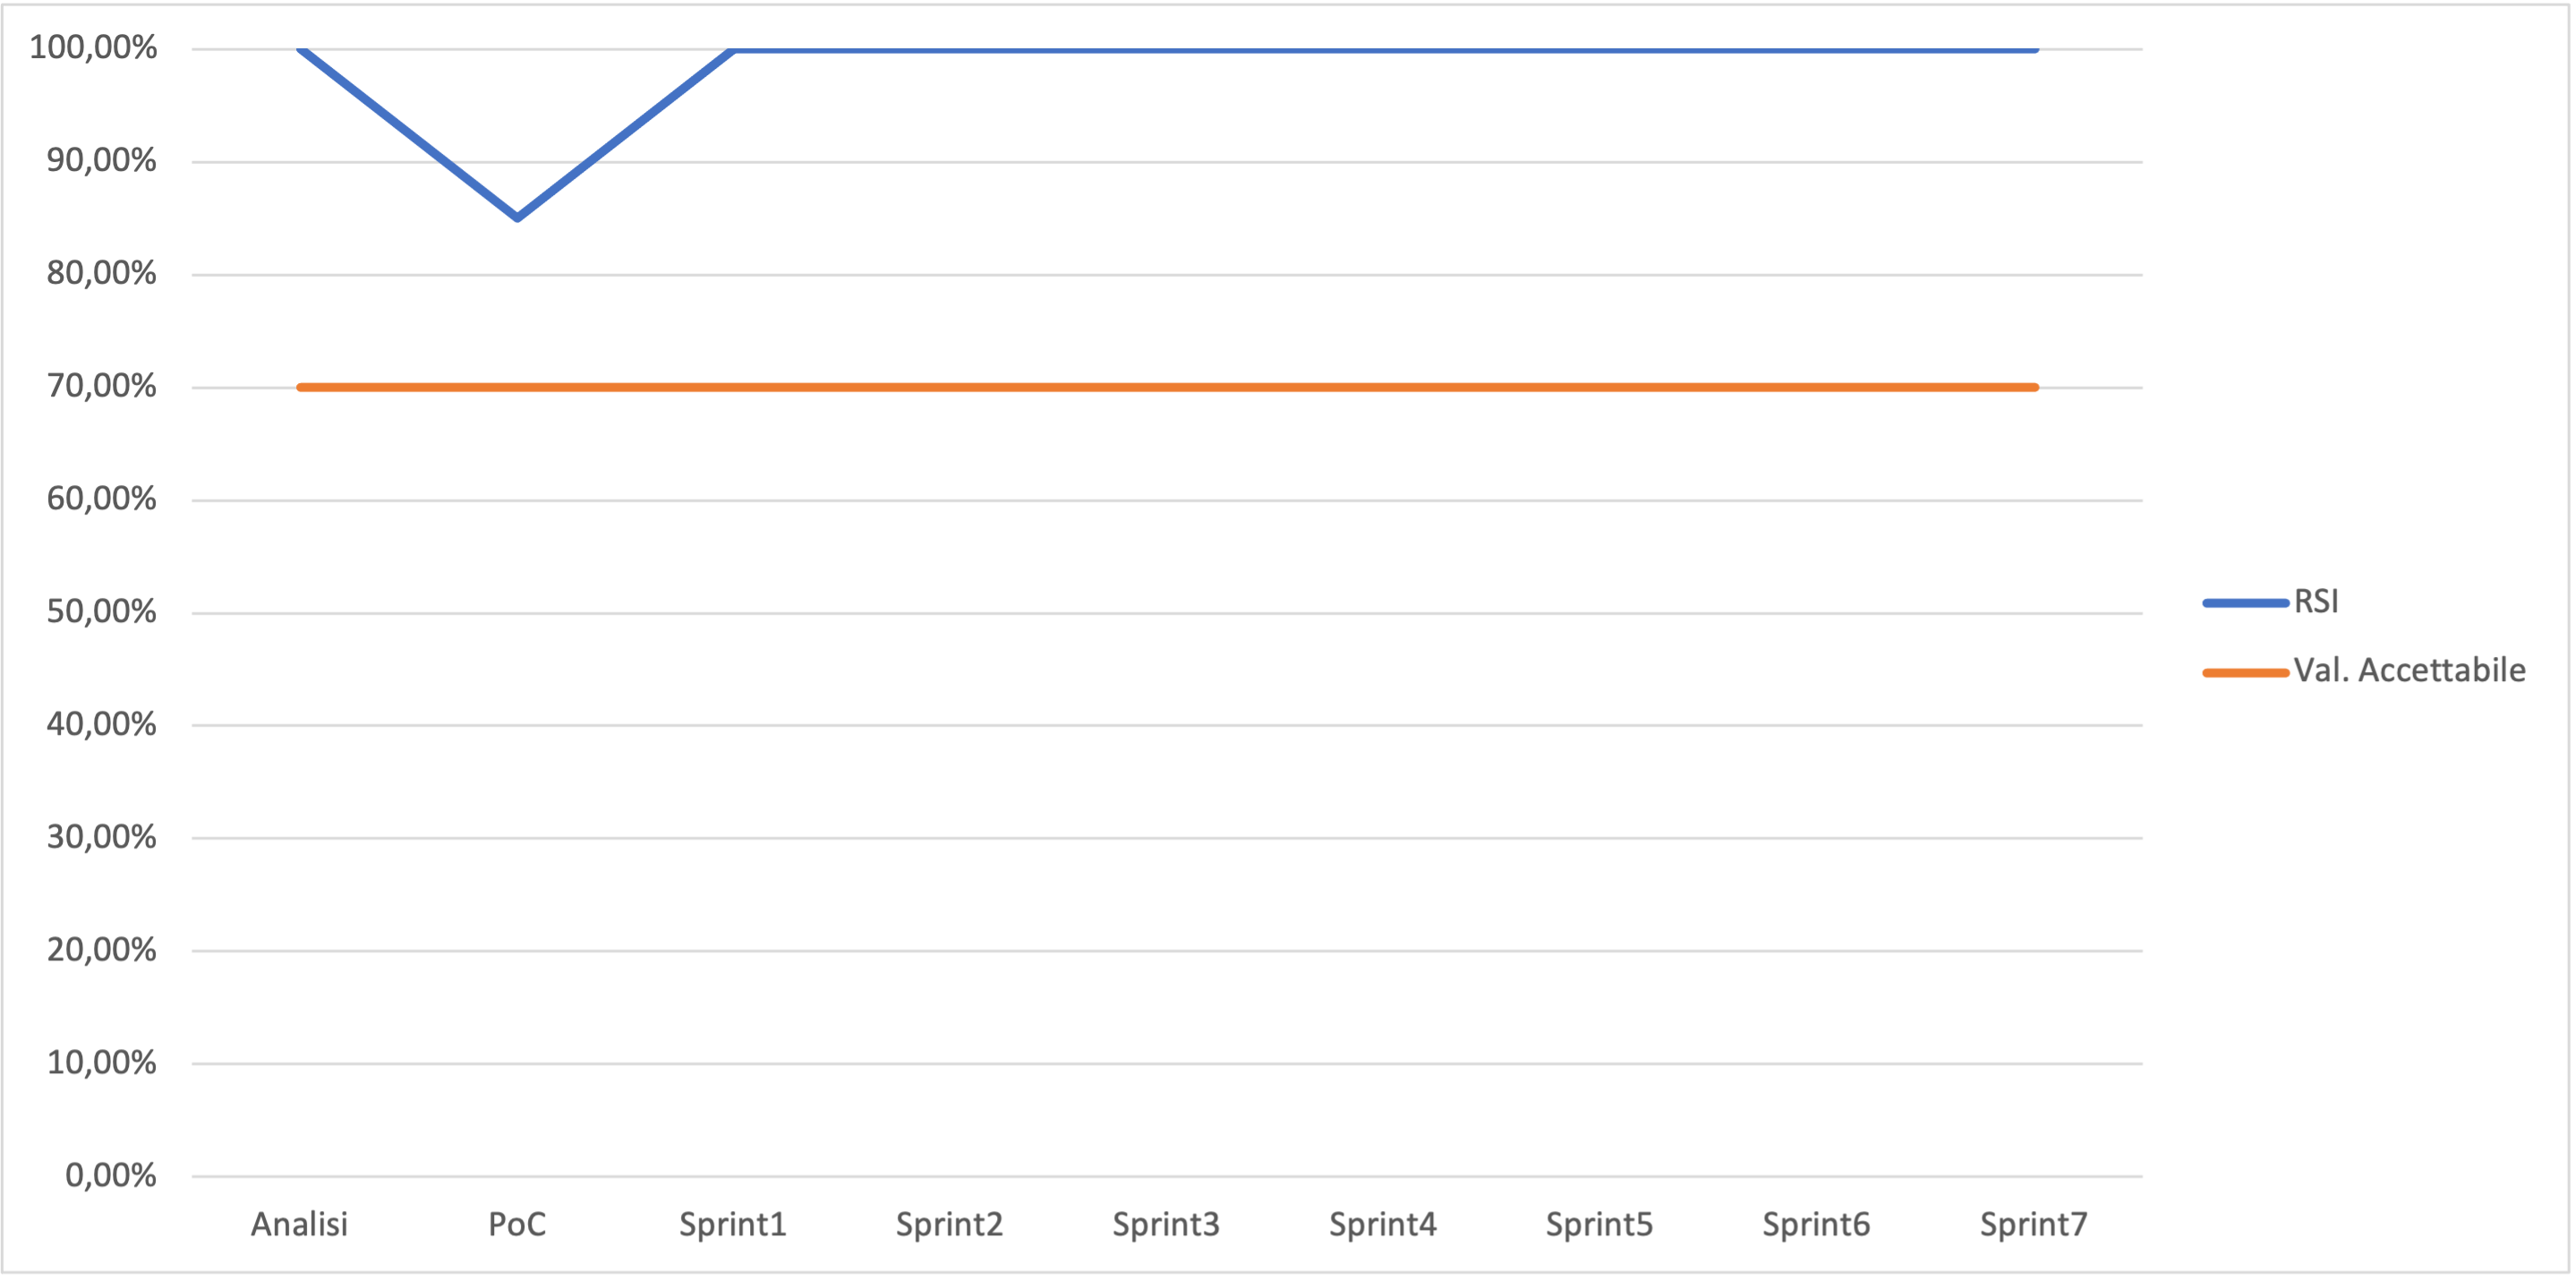
\includegraphics[width=1\textwidth]{src/img/RSI.png}
\caption{Grafico RSI}
\end{figure}

\subsubsection{Risk Found}

\begin{figure}[H]
\centering
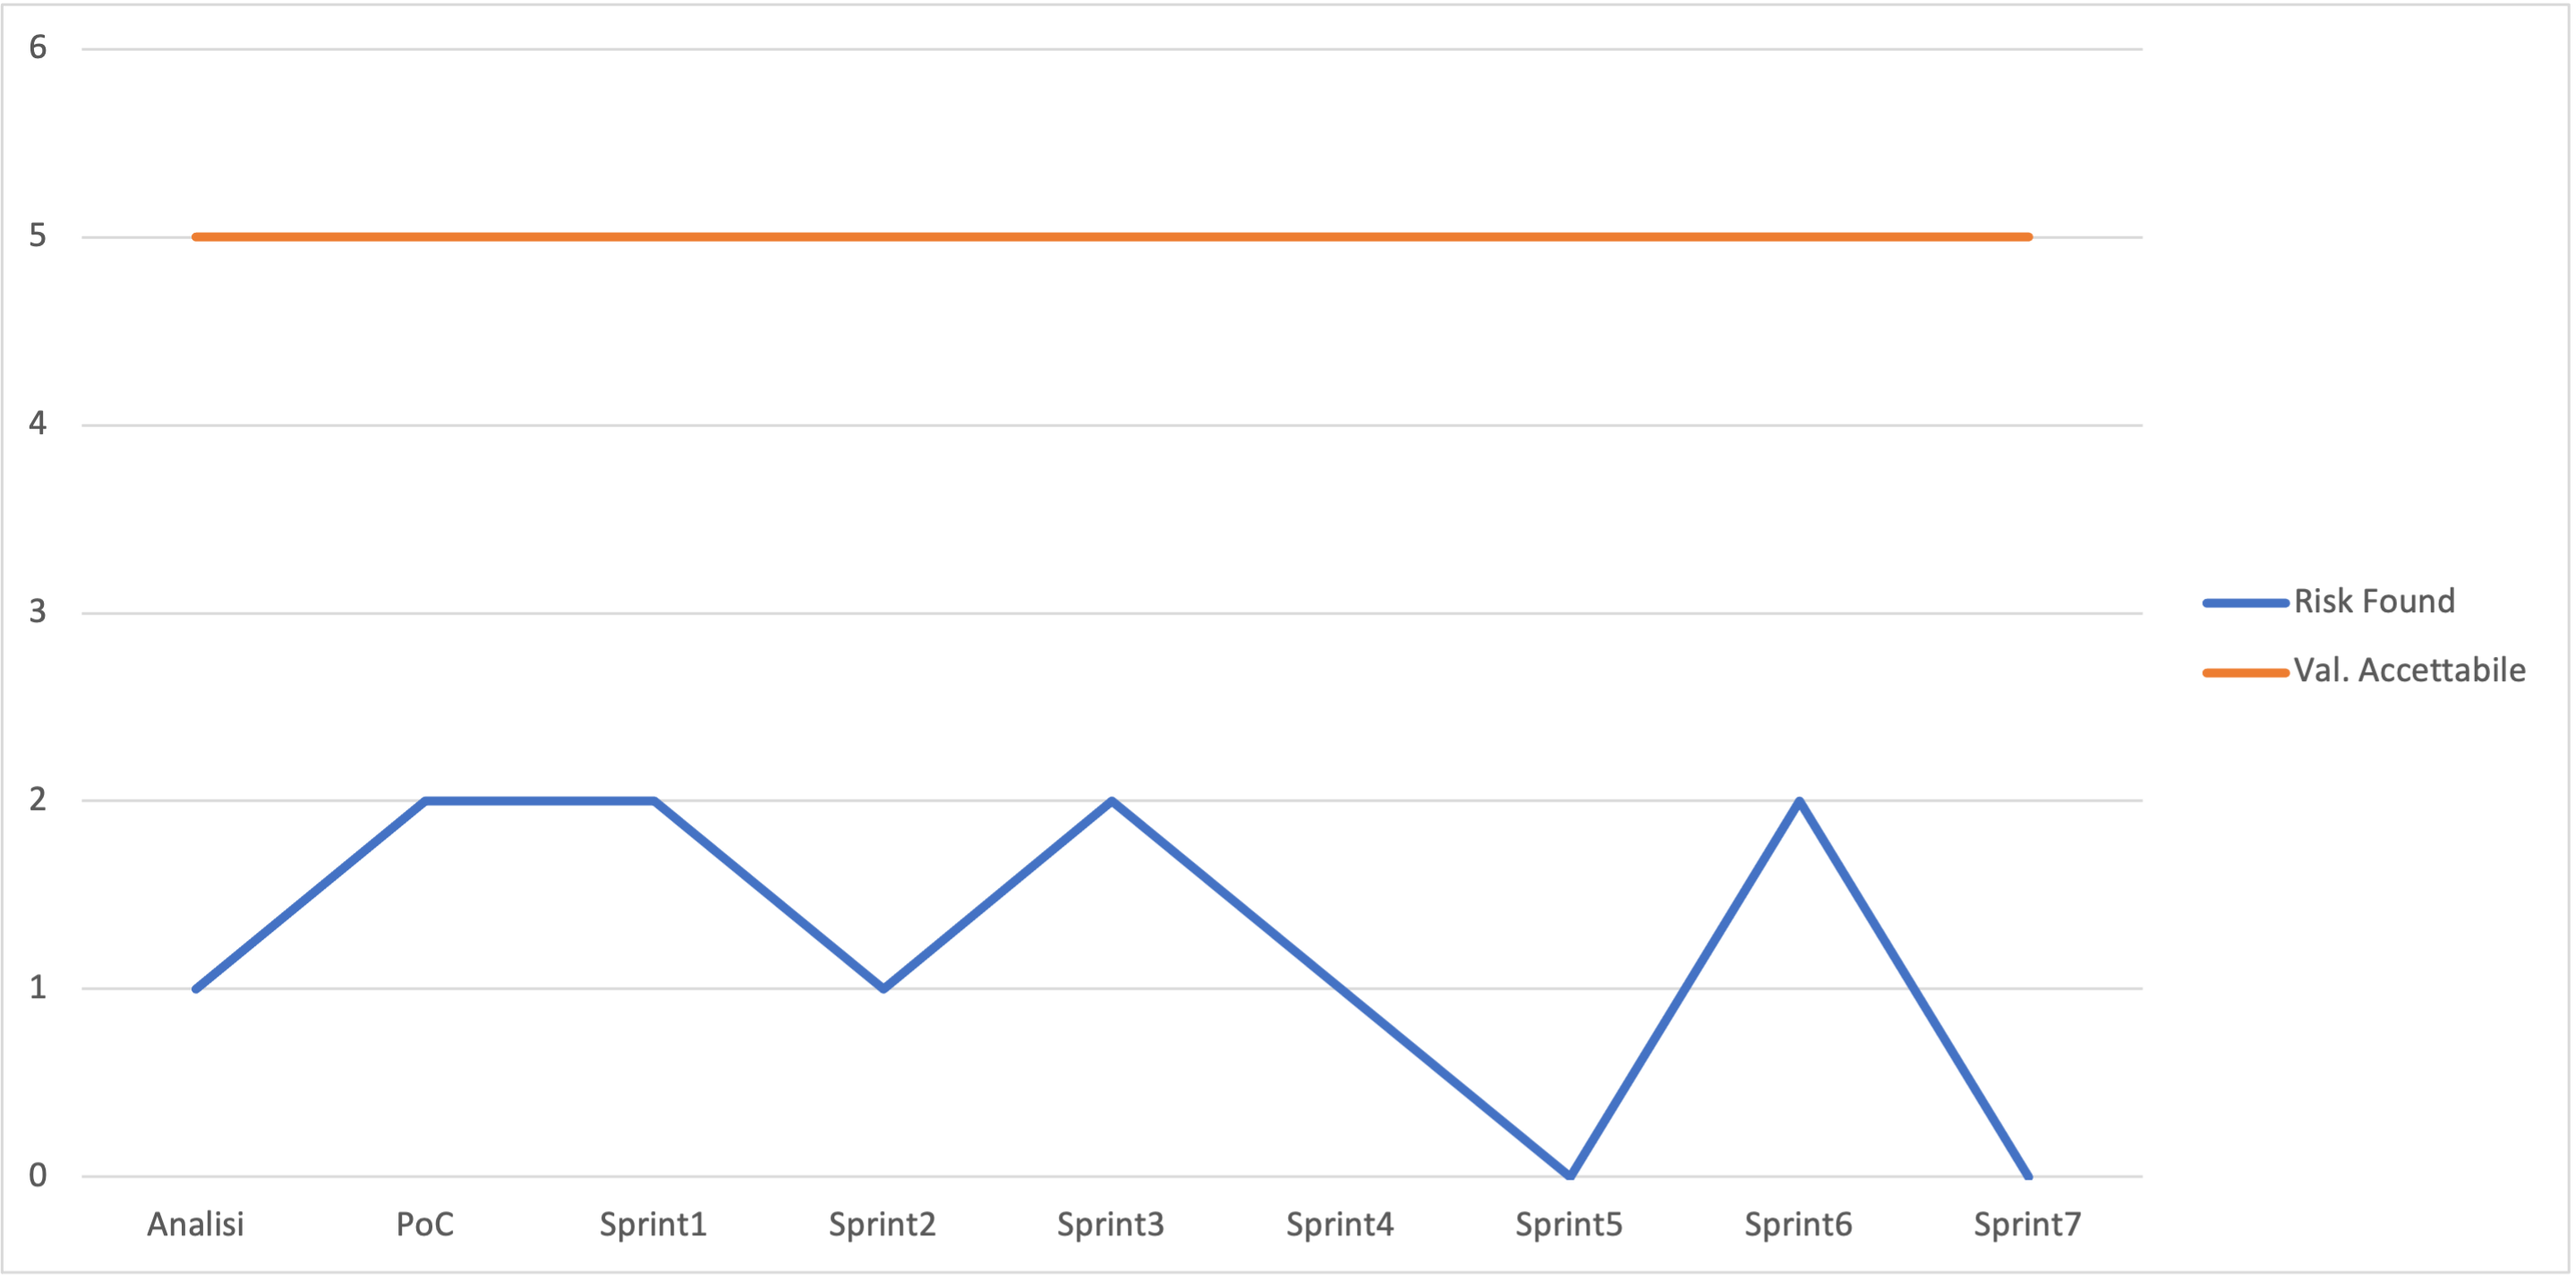
\includegraphics[width=1\textwidth]{src/img/riskFound.png}
\caption{Grafico Risk Found}
\end{figure}

\subsubsection{Metrics Satisfied}

\begin{figure}[H]
\centering
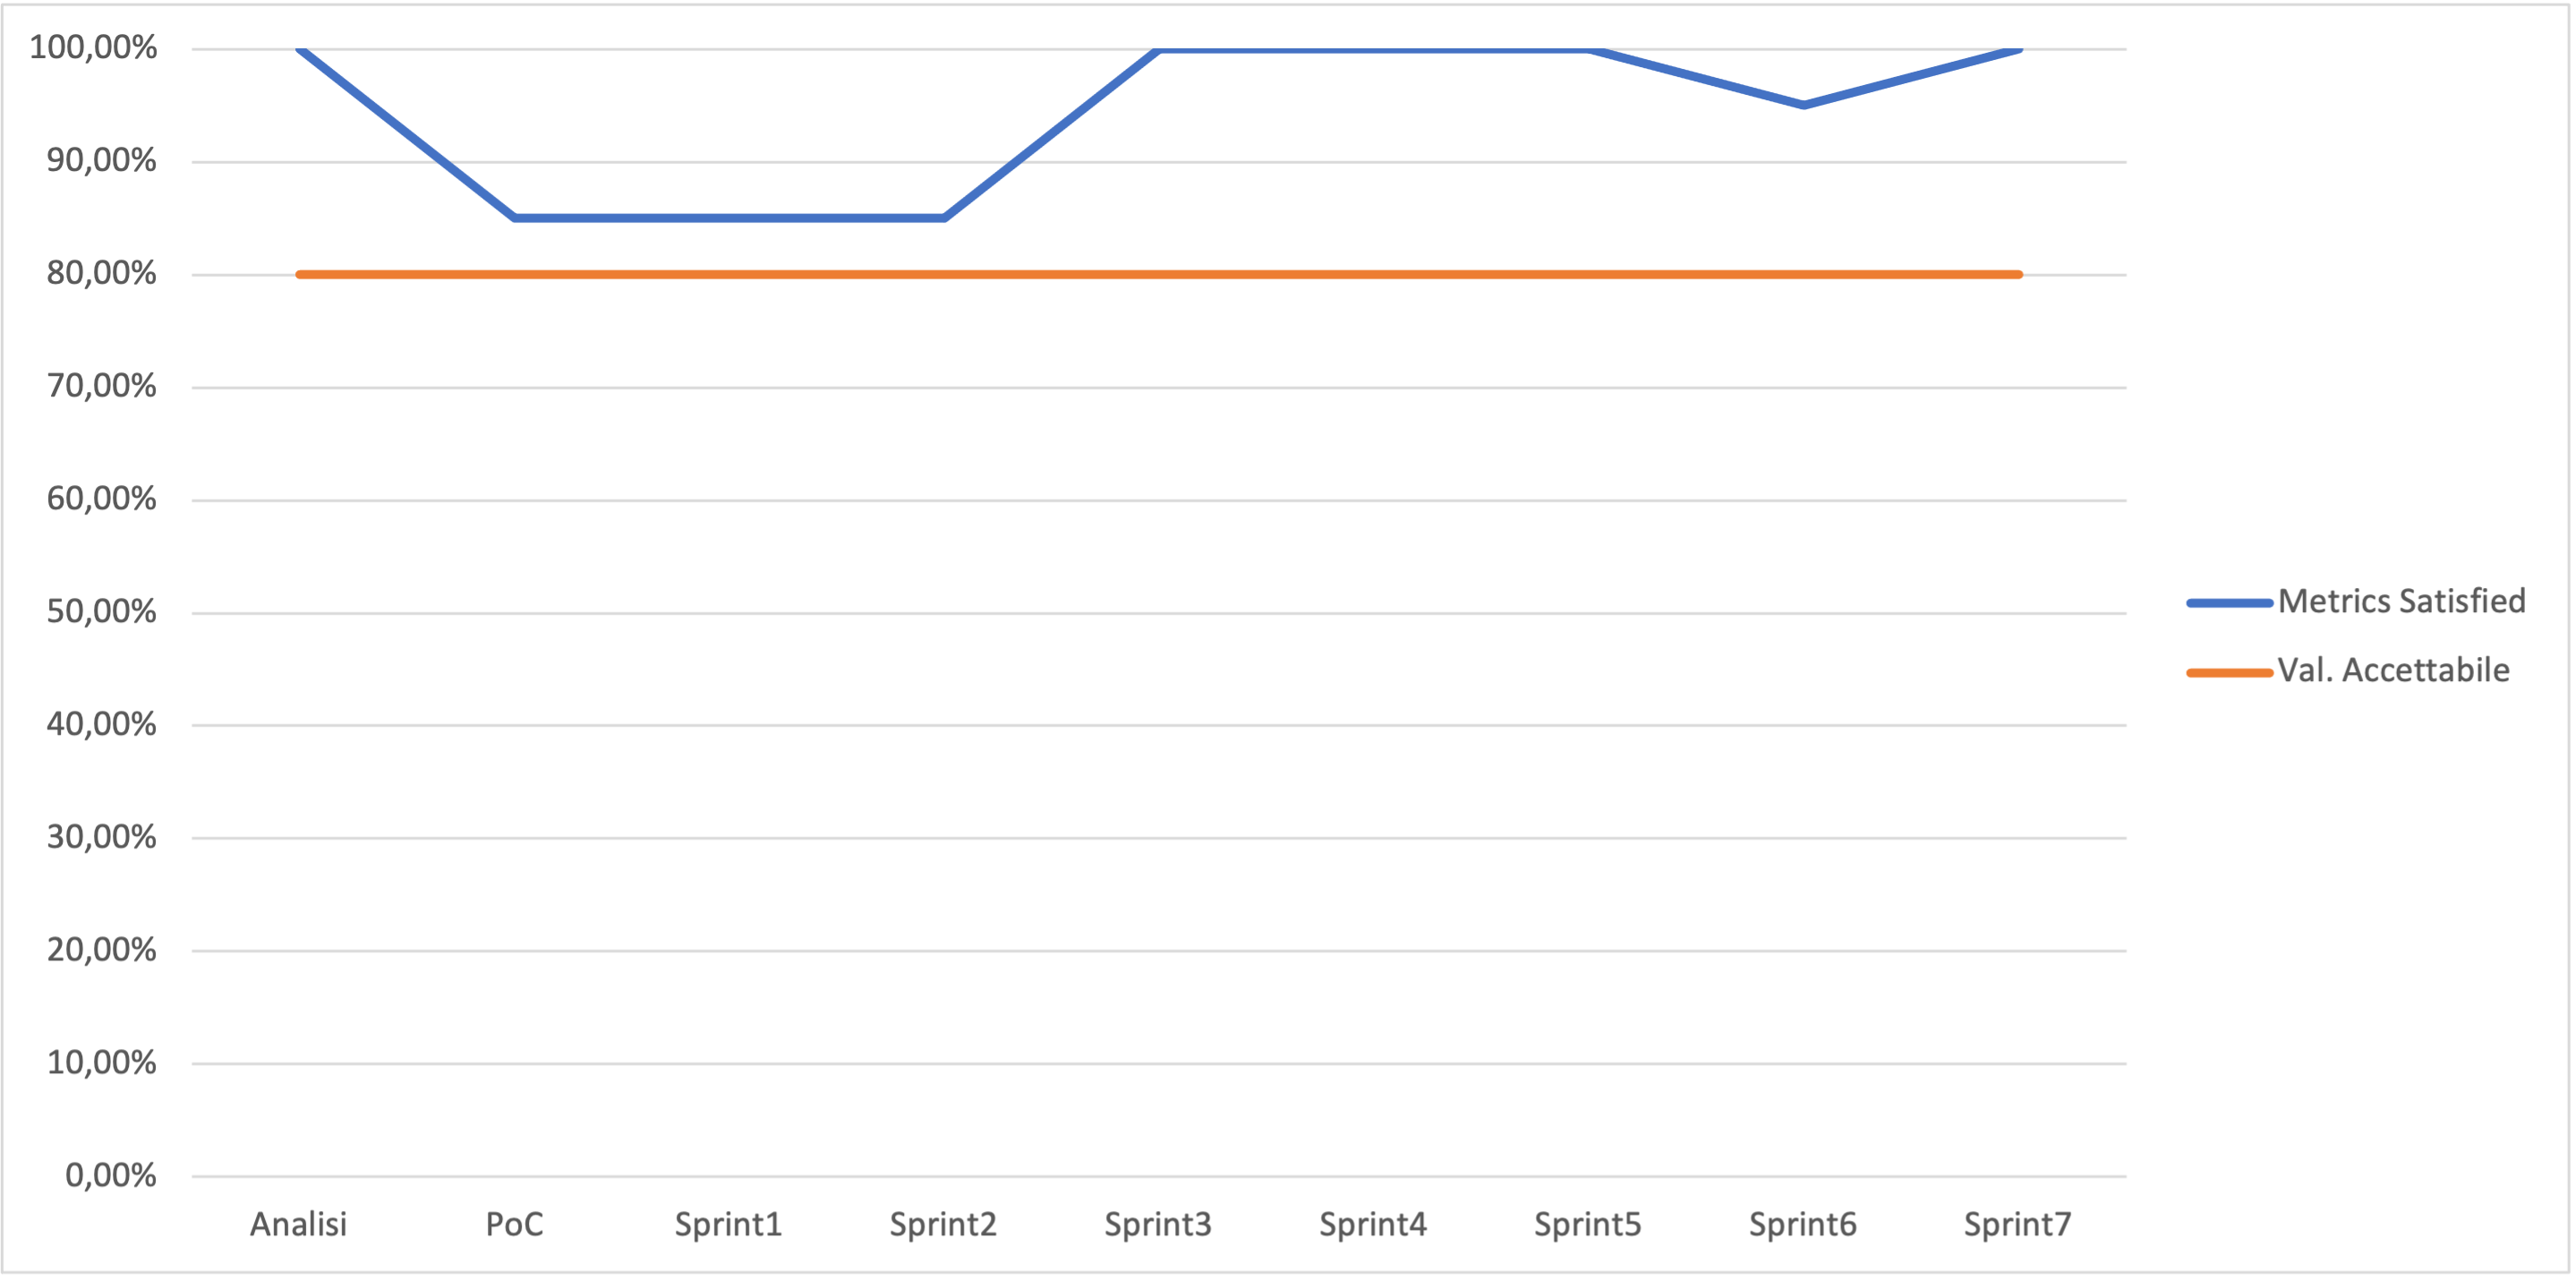
\includegraphics[width=1\textwidth]{src/img/MetricsSat.png}
\caption{Grafico Metrics Satisfied}
\end{figure}

\subsubsection{Code Coverage}

\begin{figure}[H]
\centering
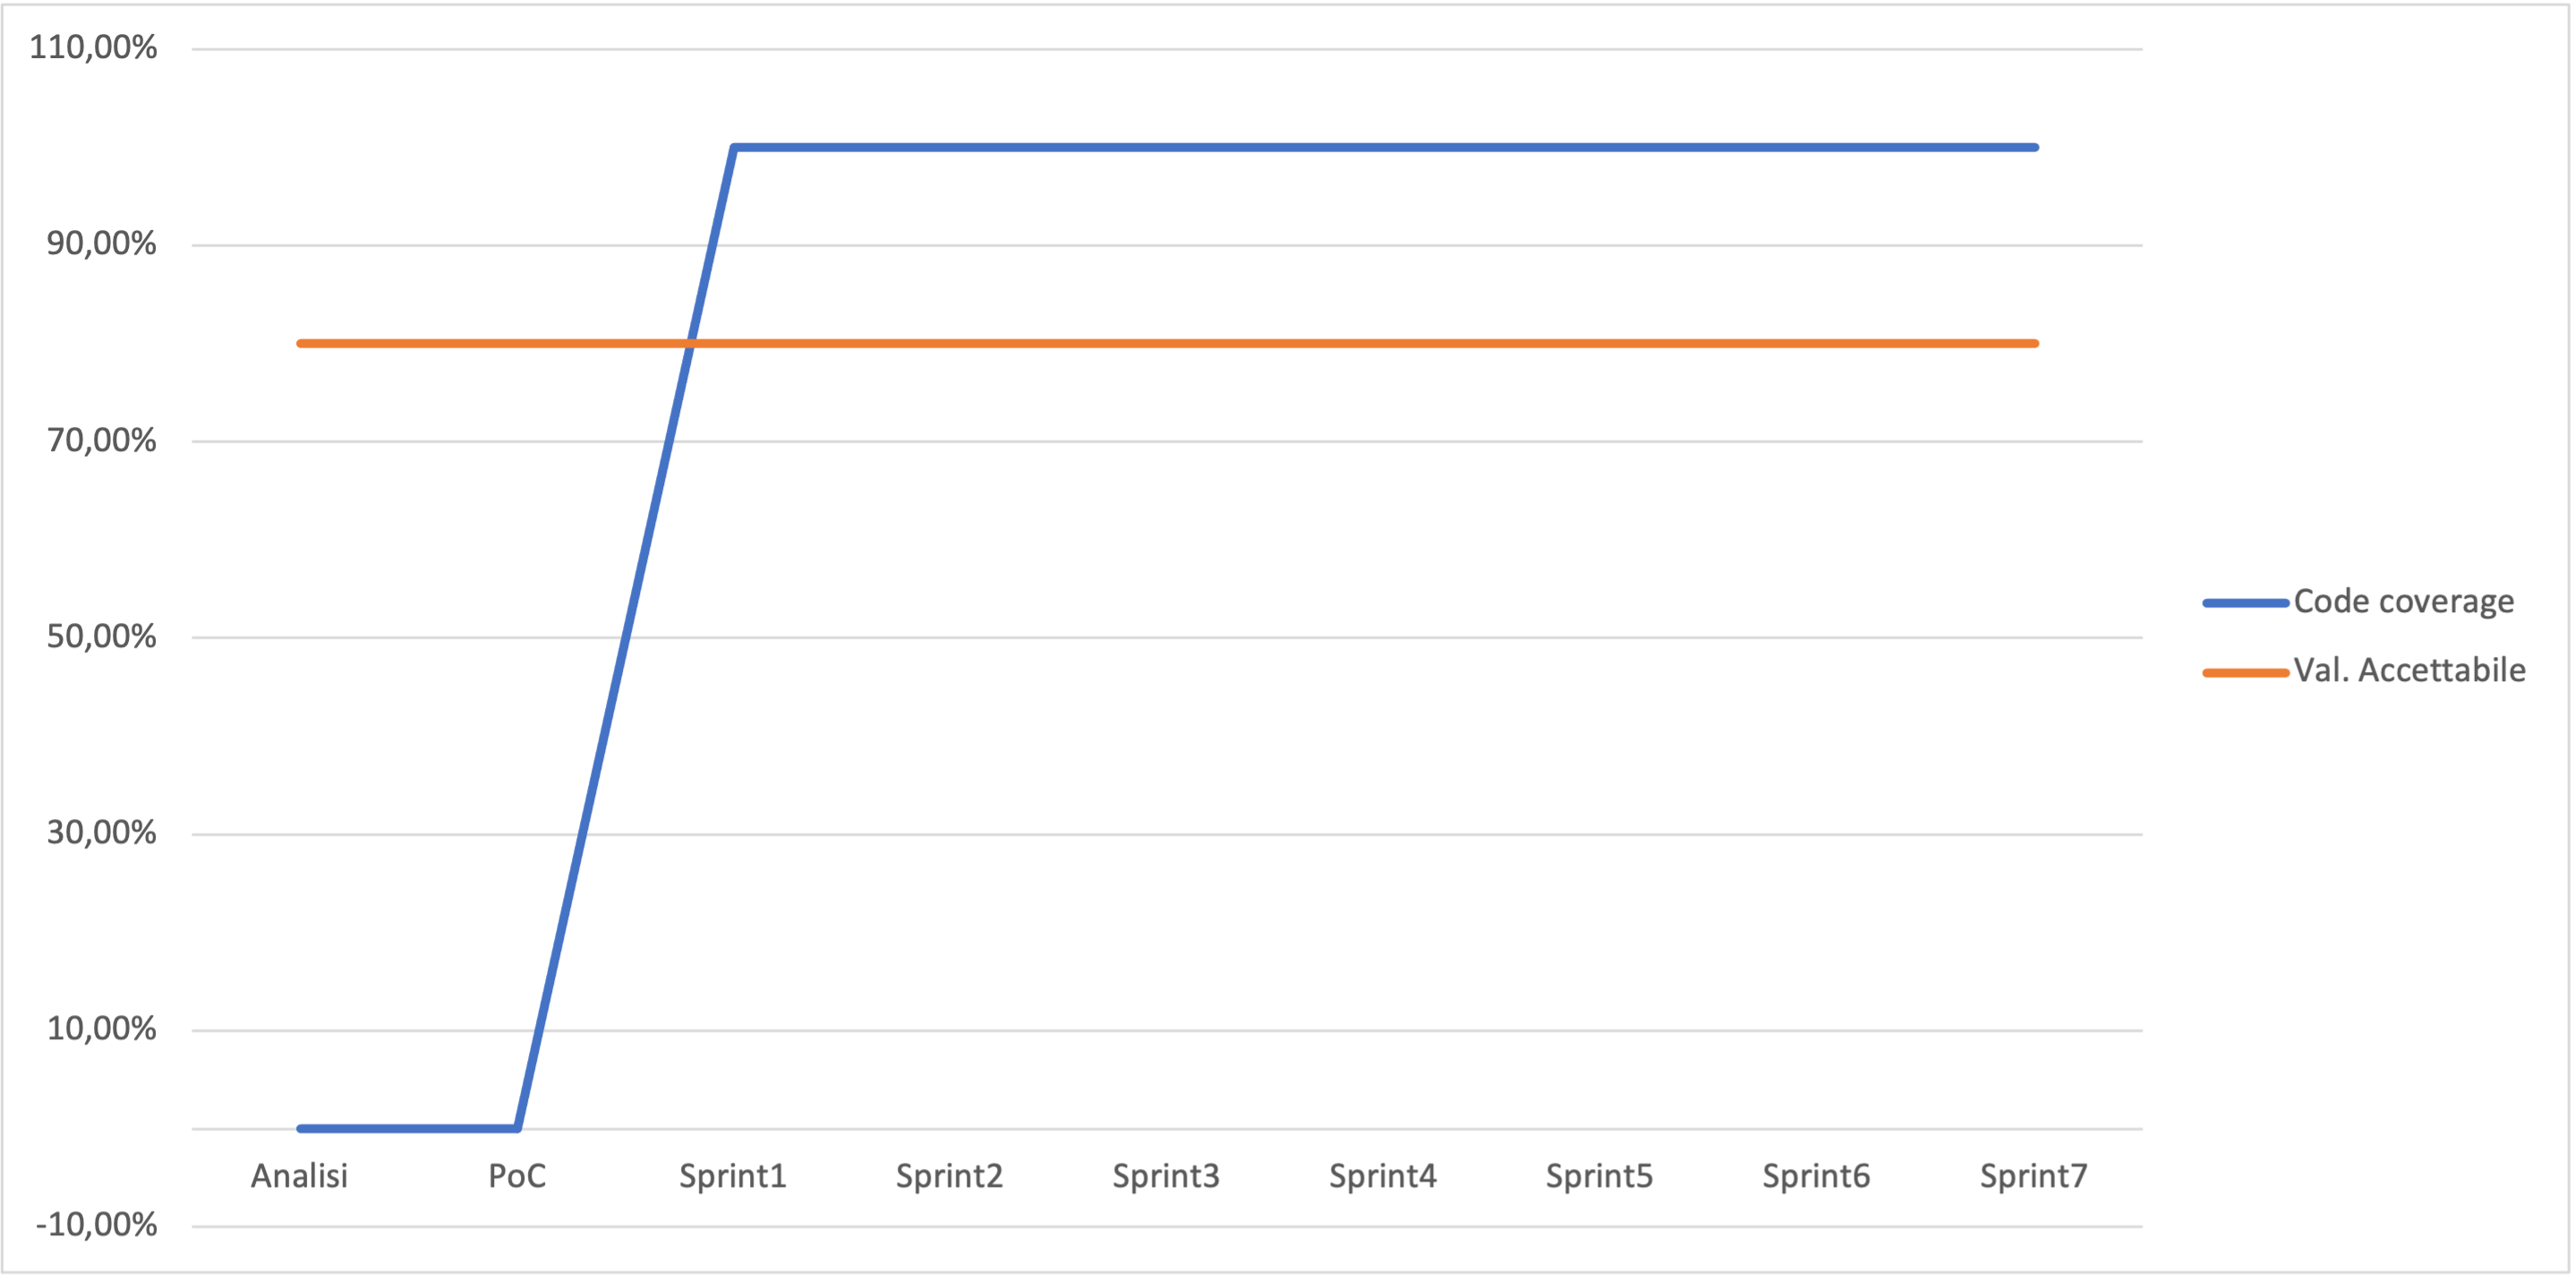
\includegraphics[width=1\textwidth]{src/img/CodeCoverage.png}
\caption{Grafico Code Coverage}
\end{figure}

\subsection{Verifica dei software}

\subsubsection{Facilità di utilizzo}

\begin{figure}[H]
\centering
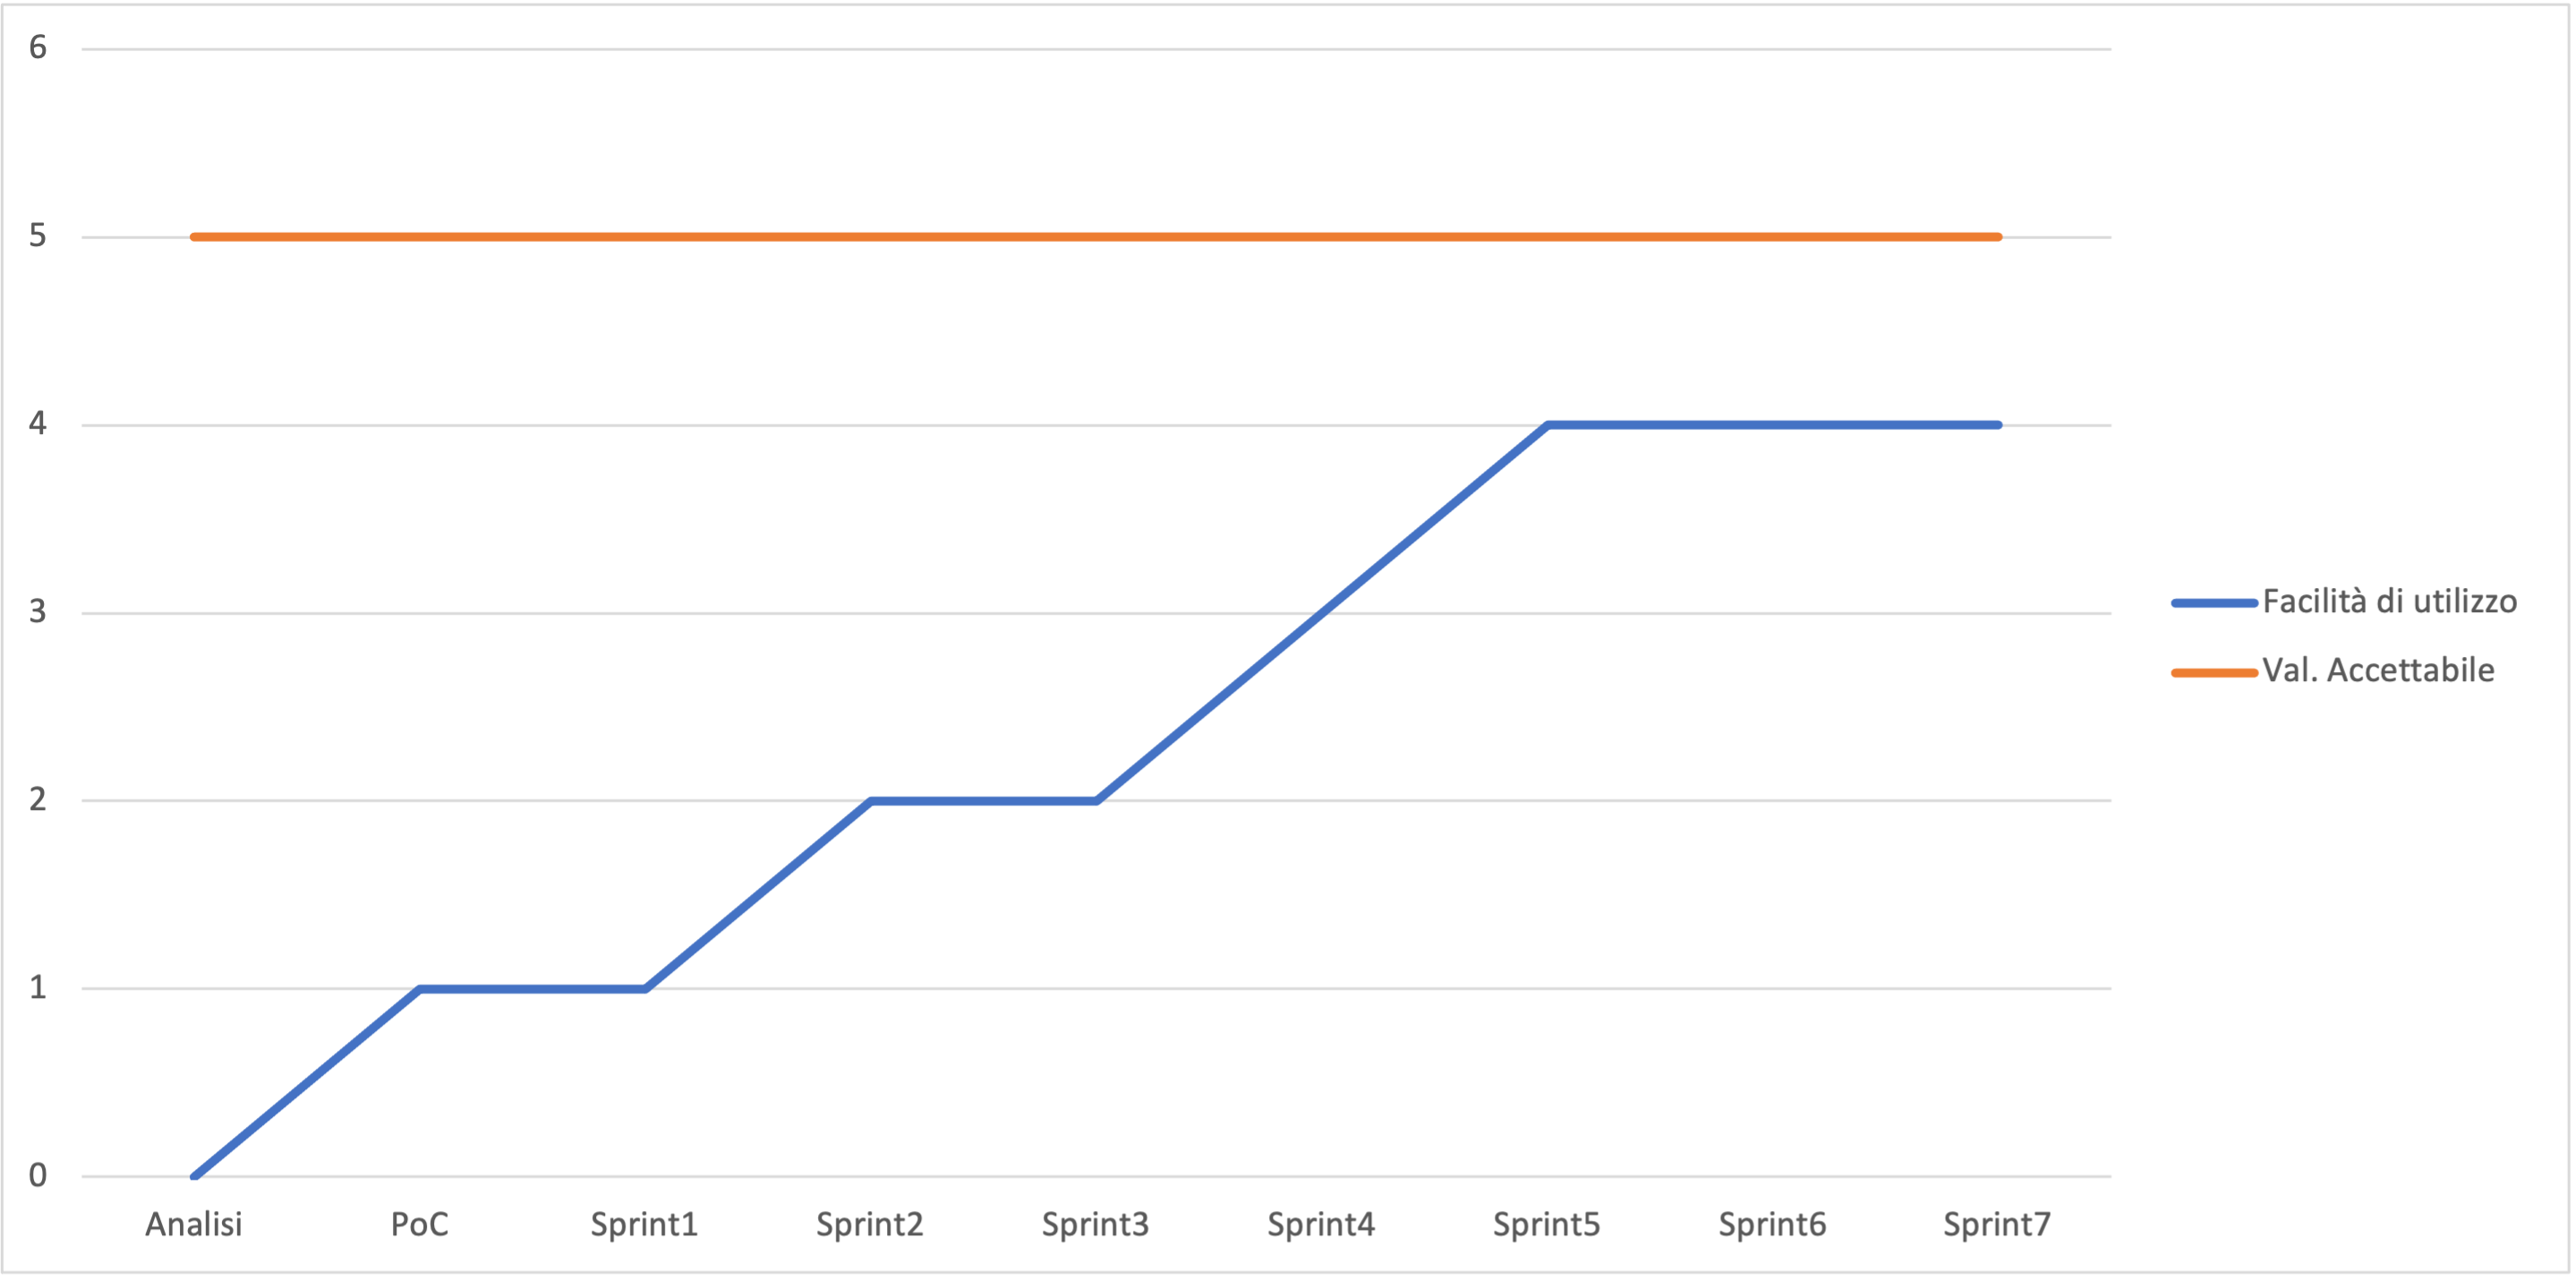
\includegraphics[width=1\textwidth]{src/img/facUtilizzo.png}
\caption{Grafico facilità di utilizzo}
\end{figure}

\subsubsection{Versioni browser supportate}

\begin{figure}[H]
\centering
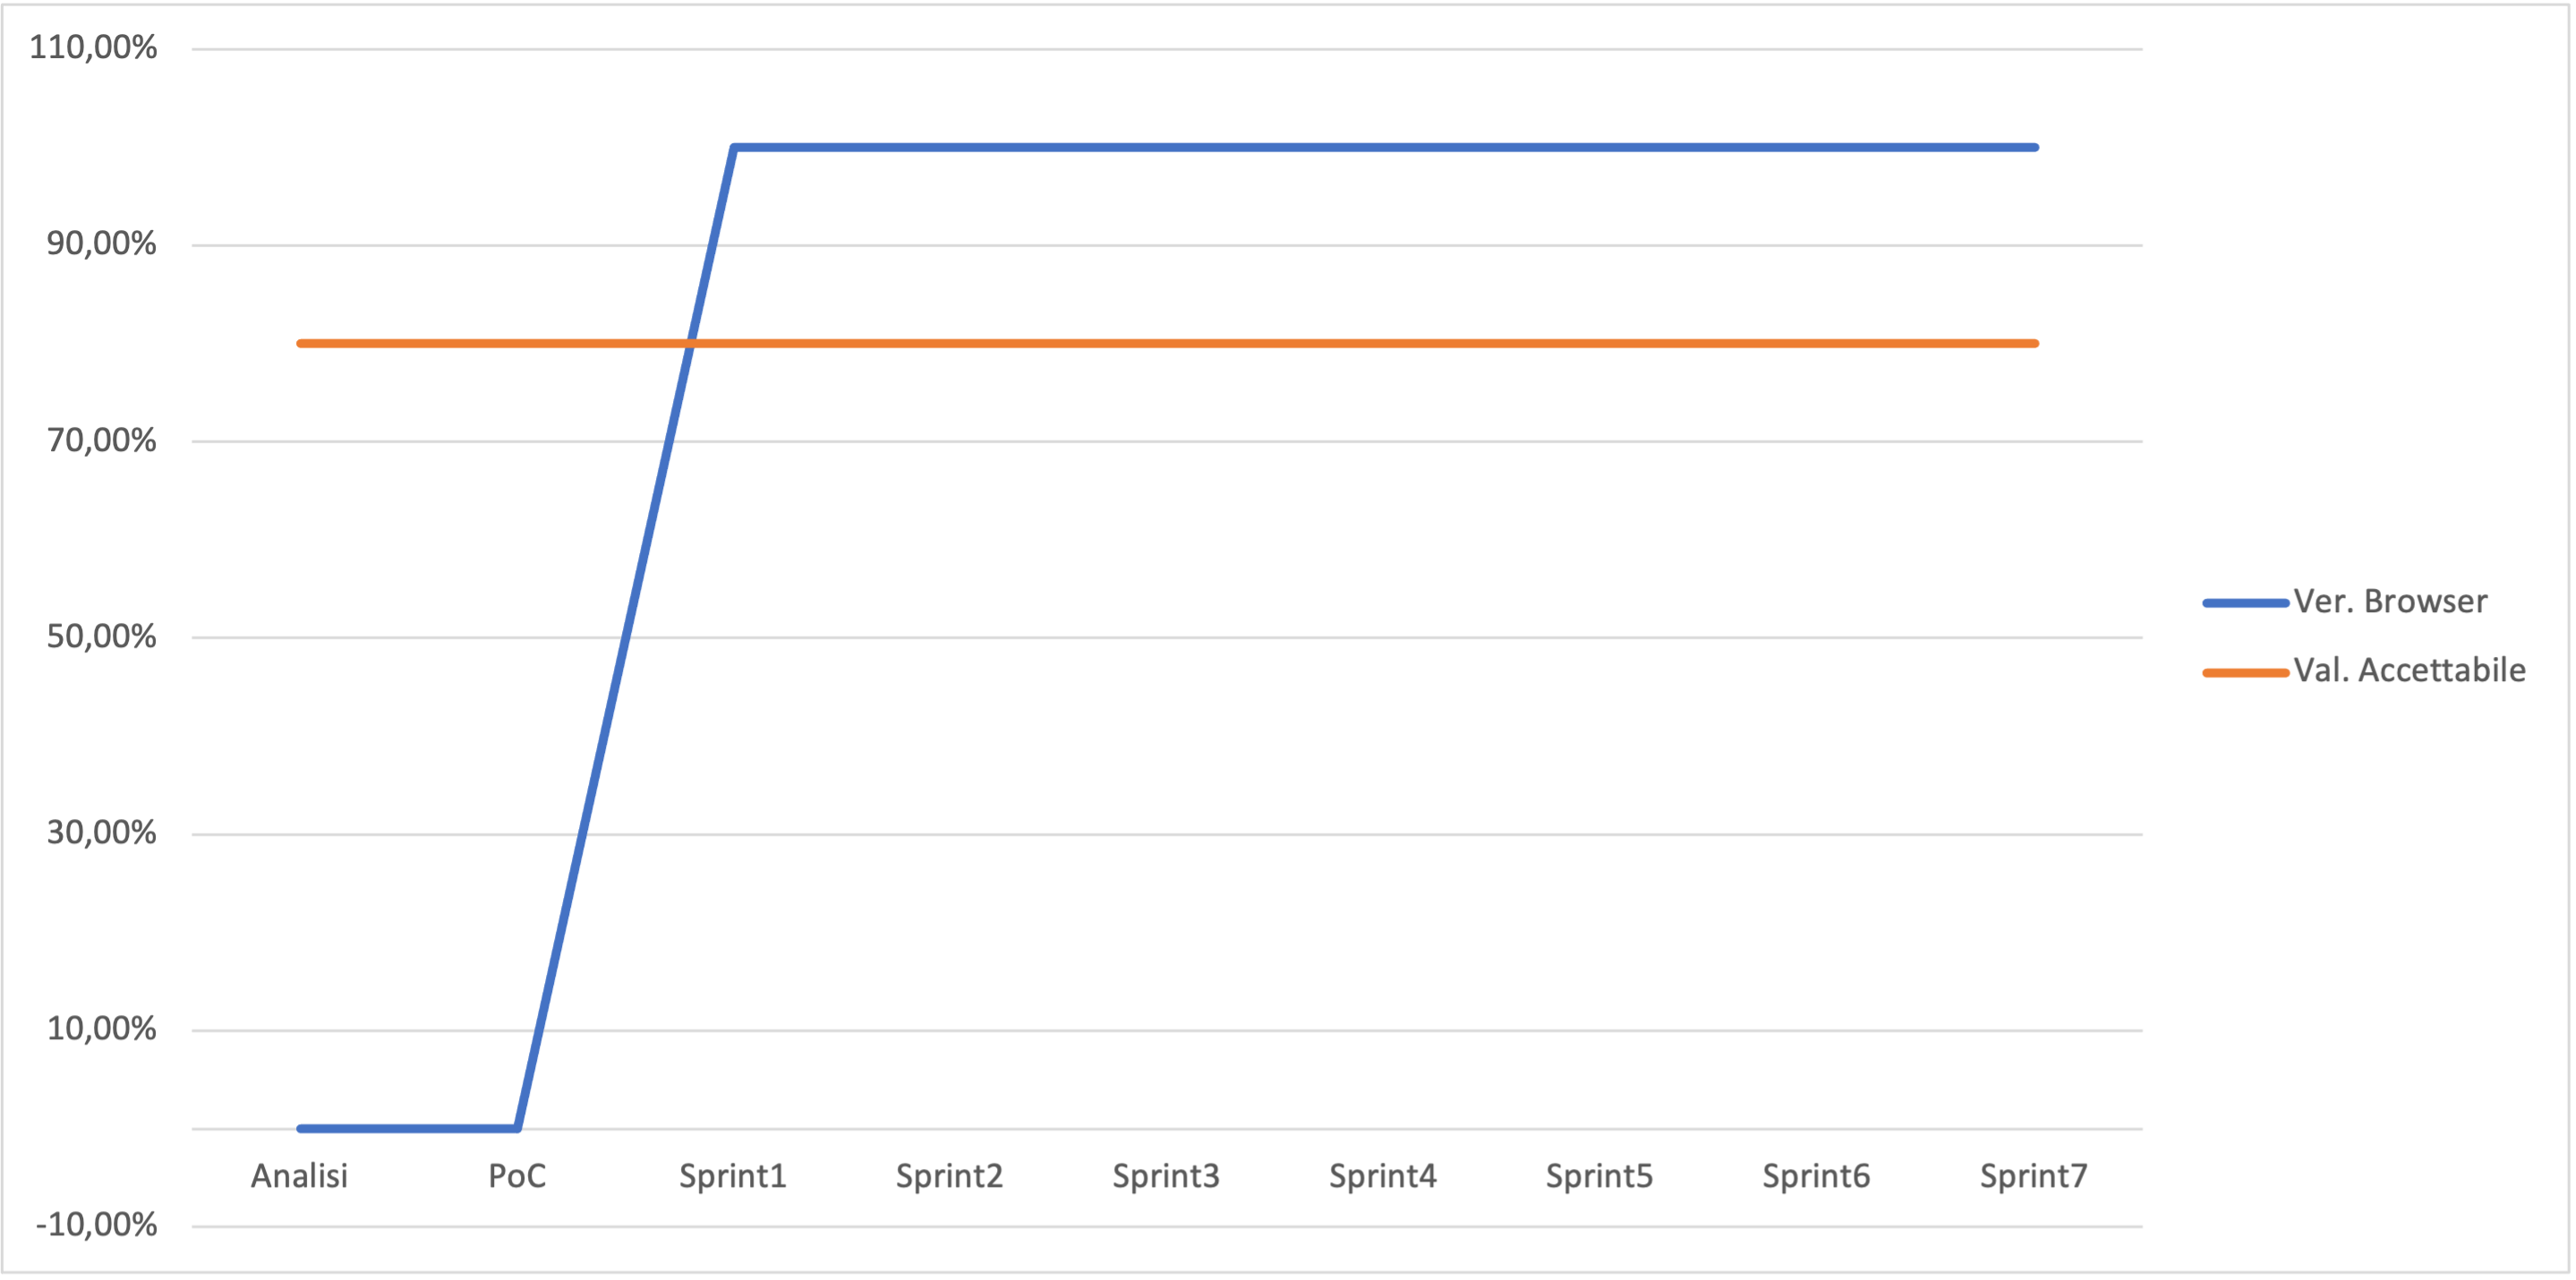
\includegraphics[width=1\textwidth]{src/img/verBrowser.png}
\caption{Grafico versioni browser supportate}
\end{figure}

\subsubsection{Mandatory Requirments Coverage}

\begin{figure}[H]
\centering
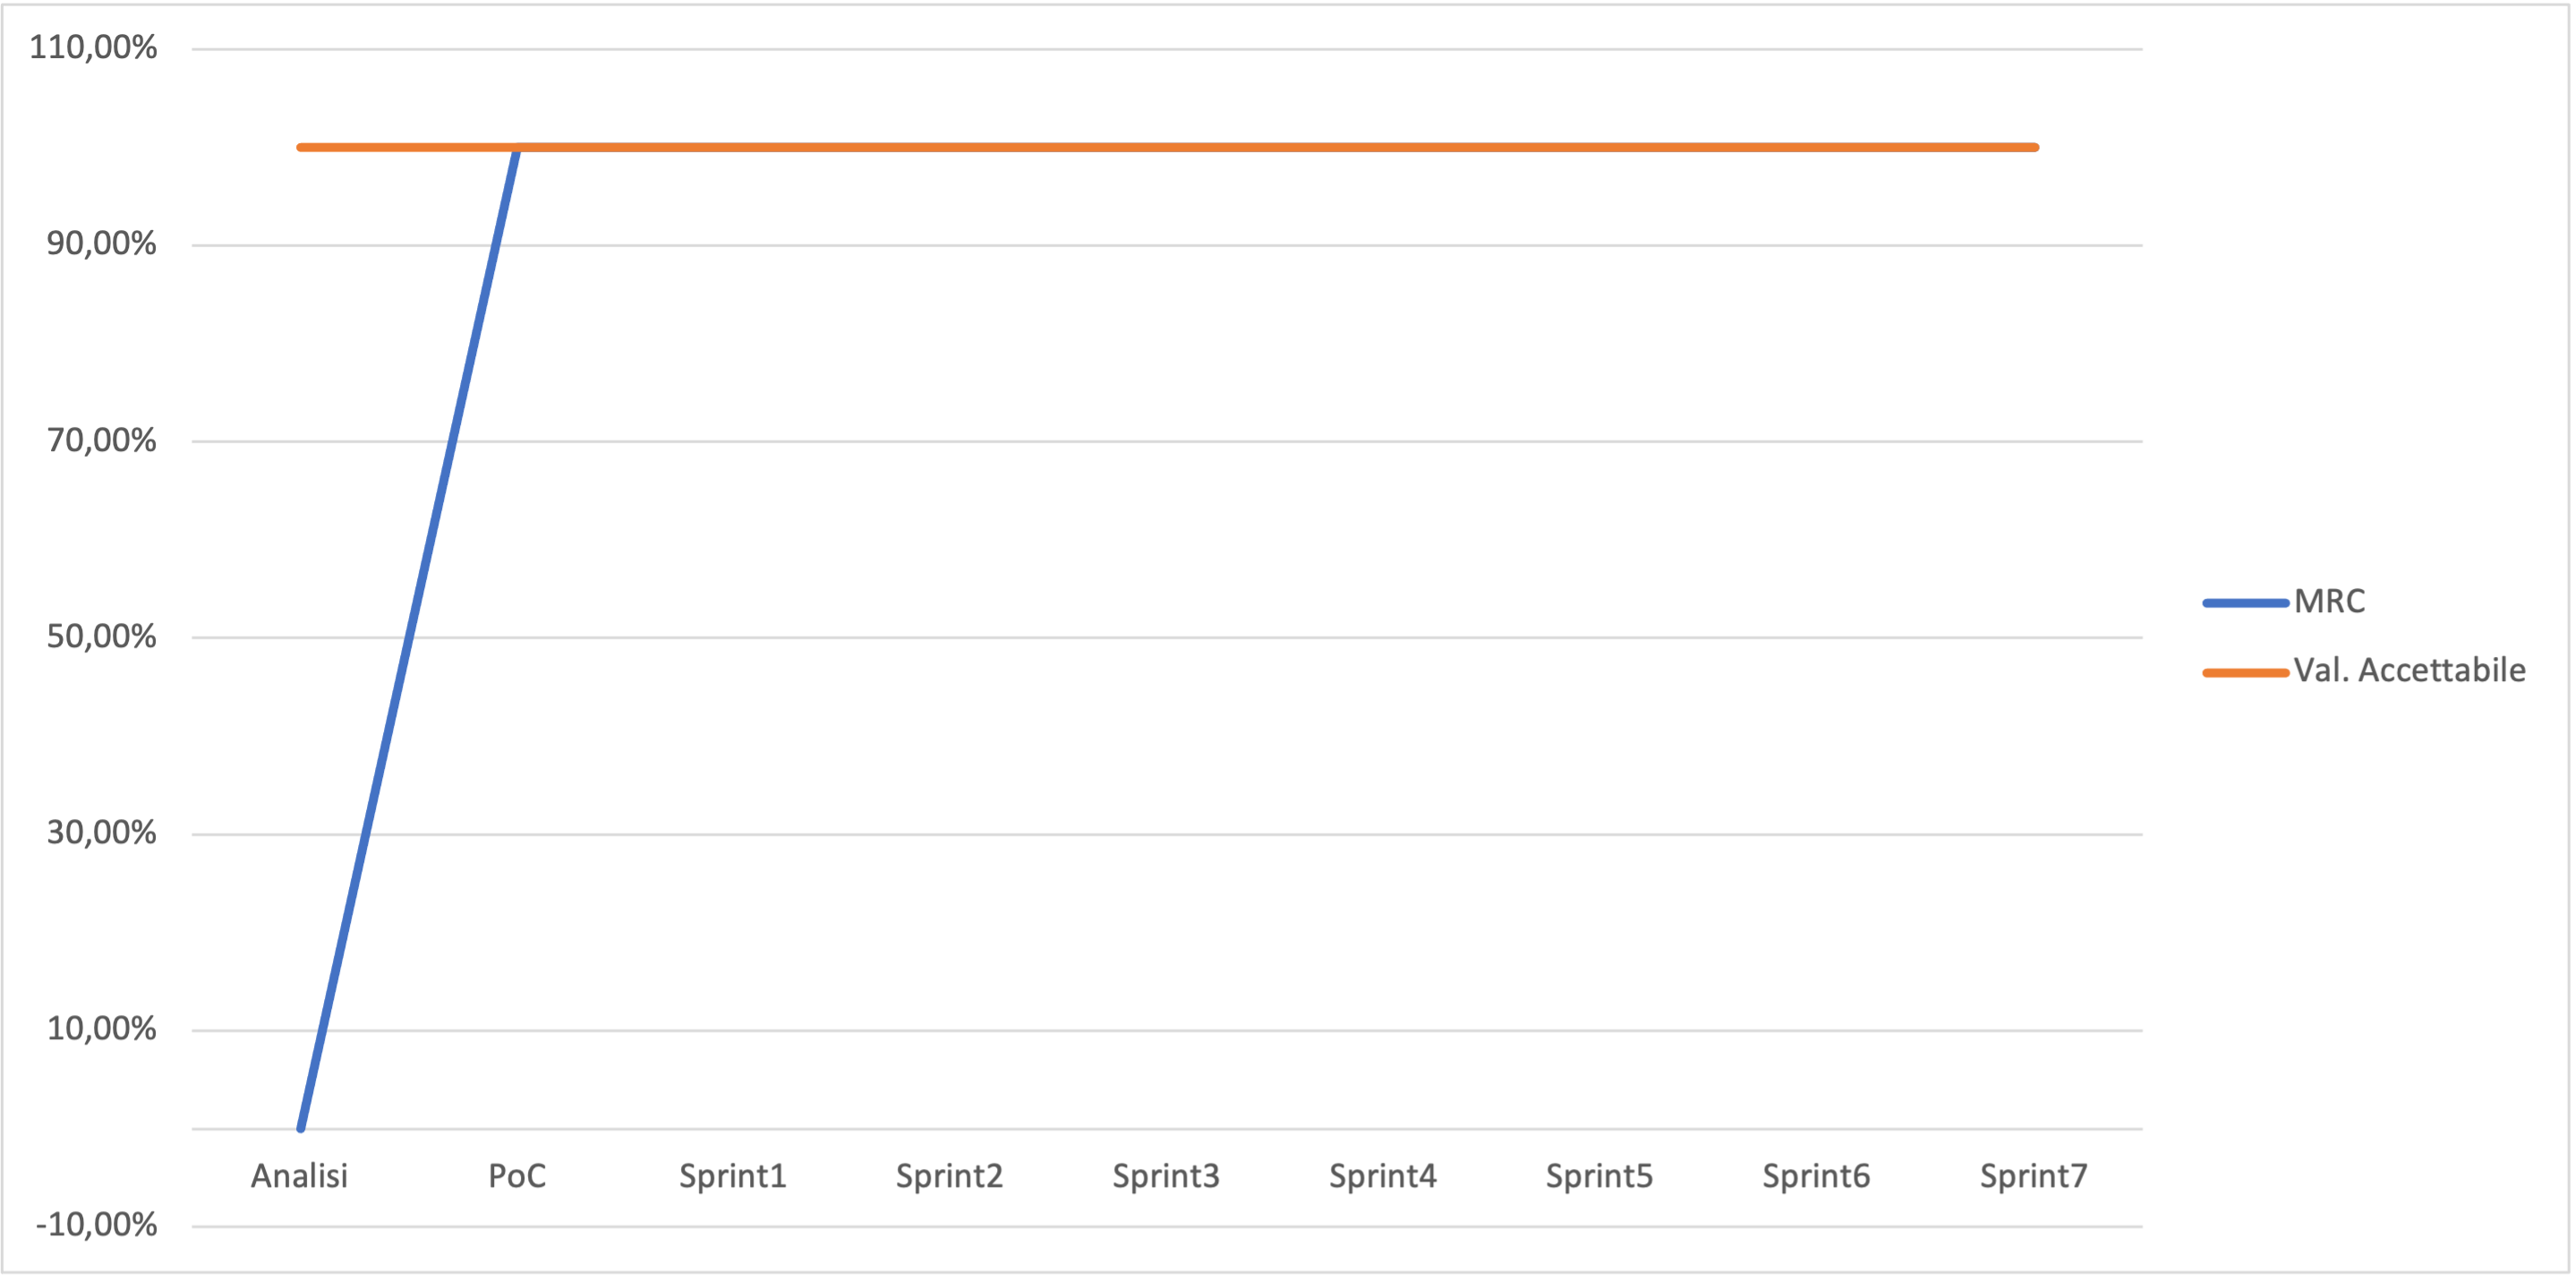
\includegraphics[width=1\textwidth]{src/img/MRC.png}
\caption{Grafico MRC}
\end{figure}

\subsubsection{Desirable Requirments Coverage}

\begin{figure}[H]
\centering
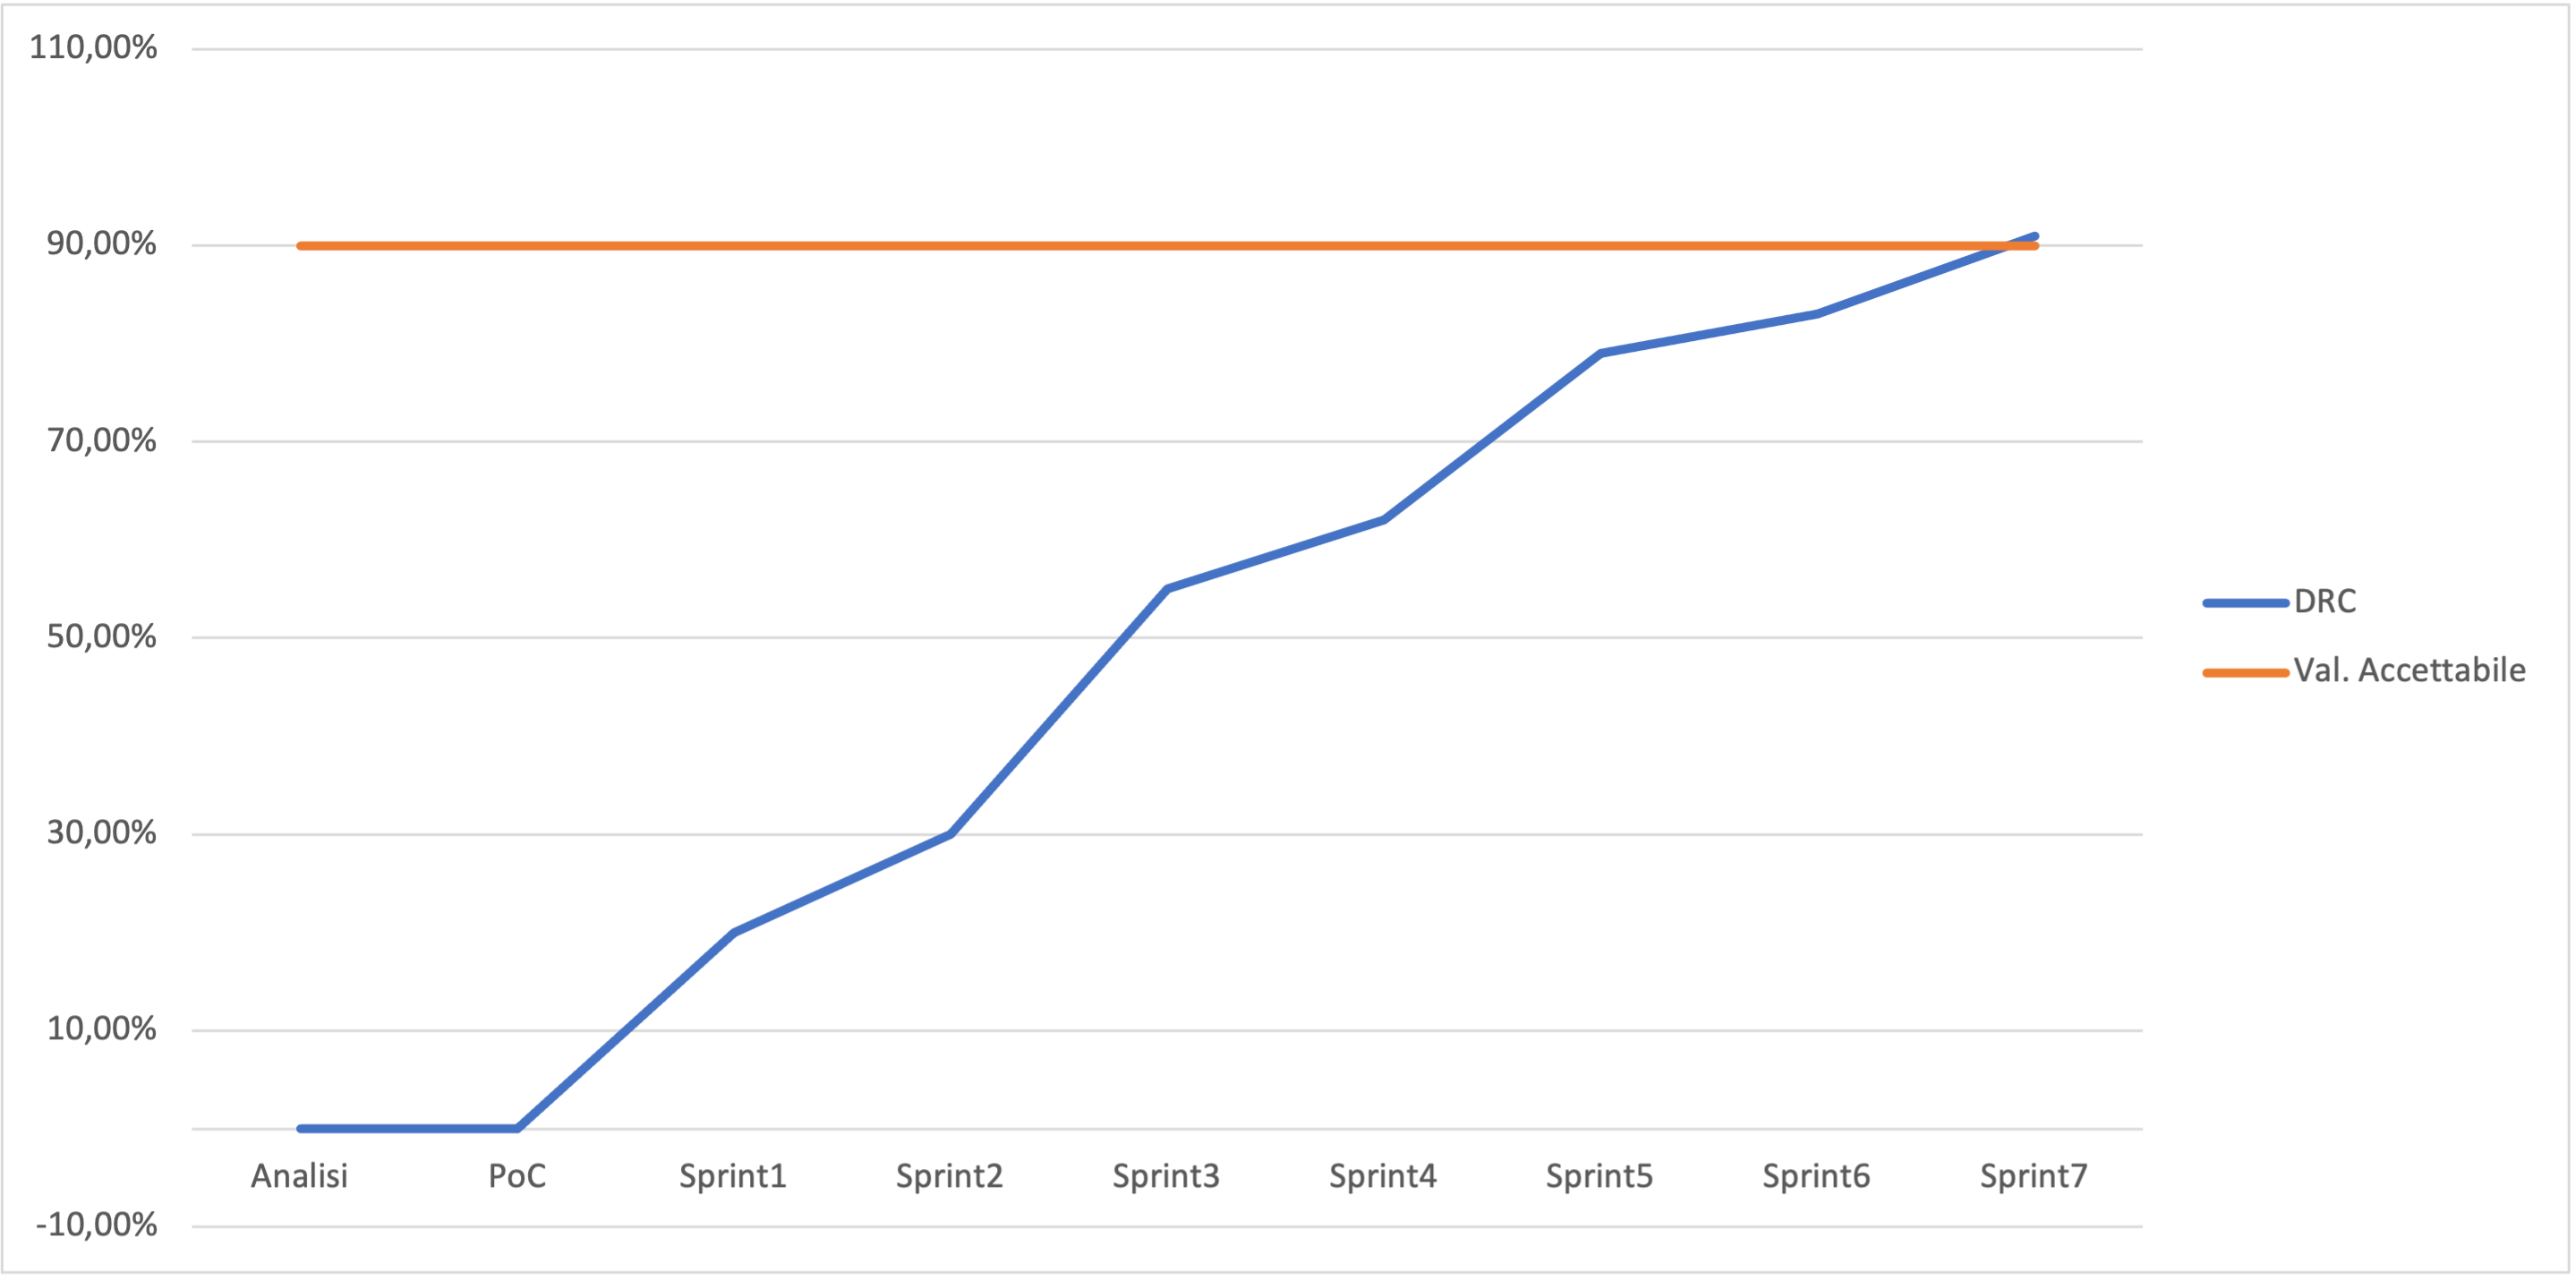
\includegraphics[width=1\textwidth]{src/img/DRC.png}
\caption{Grafico DRC}
\end{figure}

\subsubsection{Optional Requirments Coverage}

\begin{figure}[H]
\centering
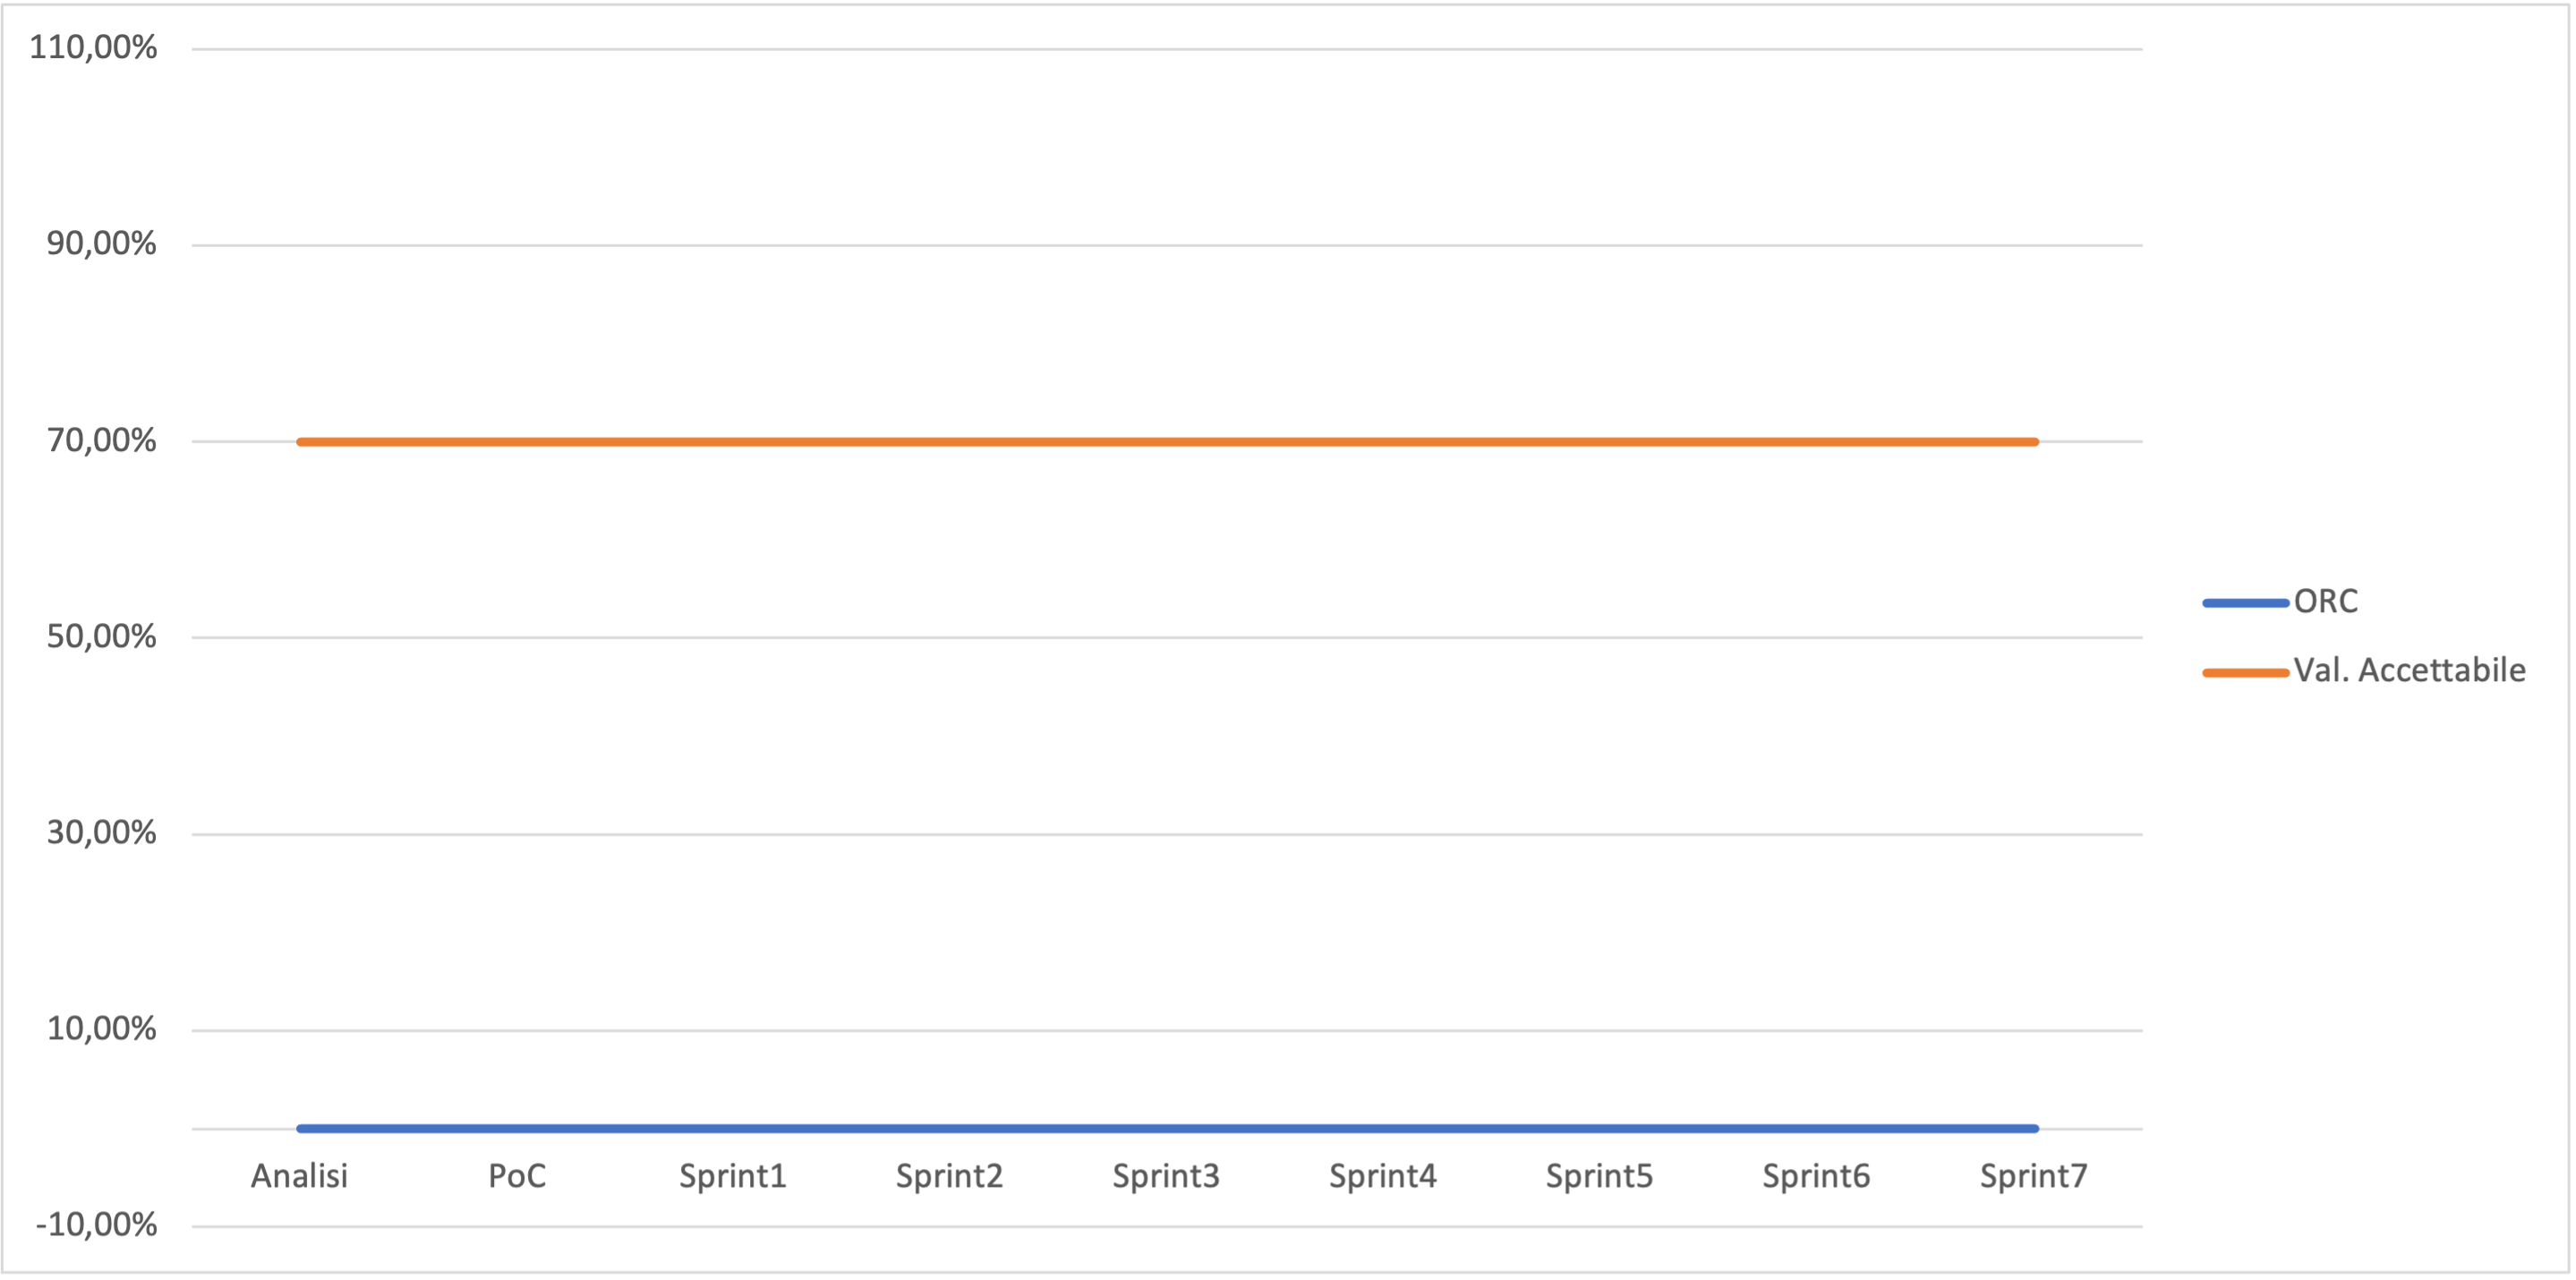
\includegraphics[width=1\textwidth]{src/img/ORC.png}
\caption{Grafico ORC}
\end{figure}

\subsubsection{Solidity Statement Coverage}

\begin{figure}[H]
\centering
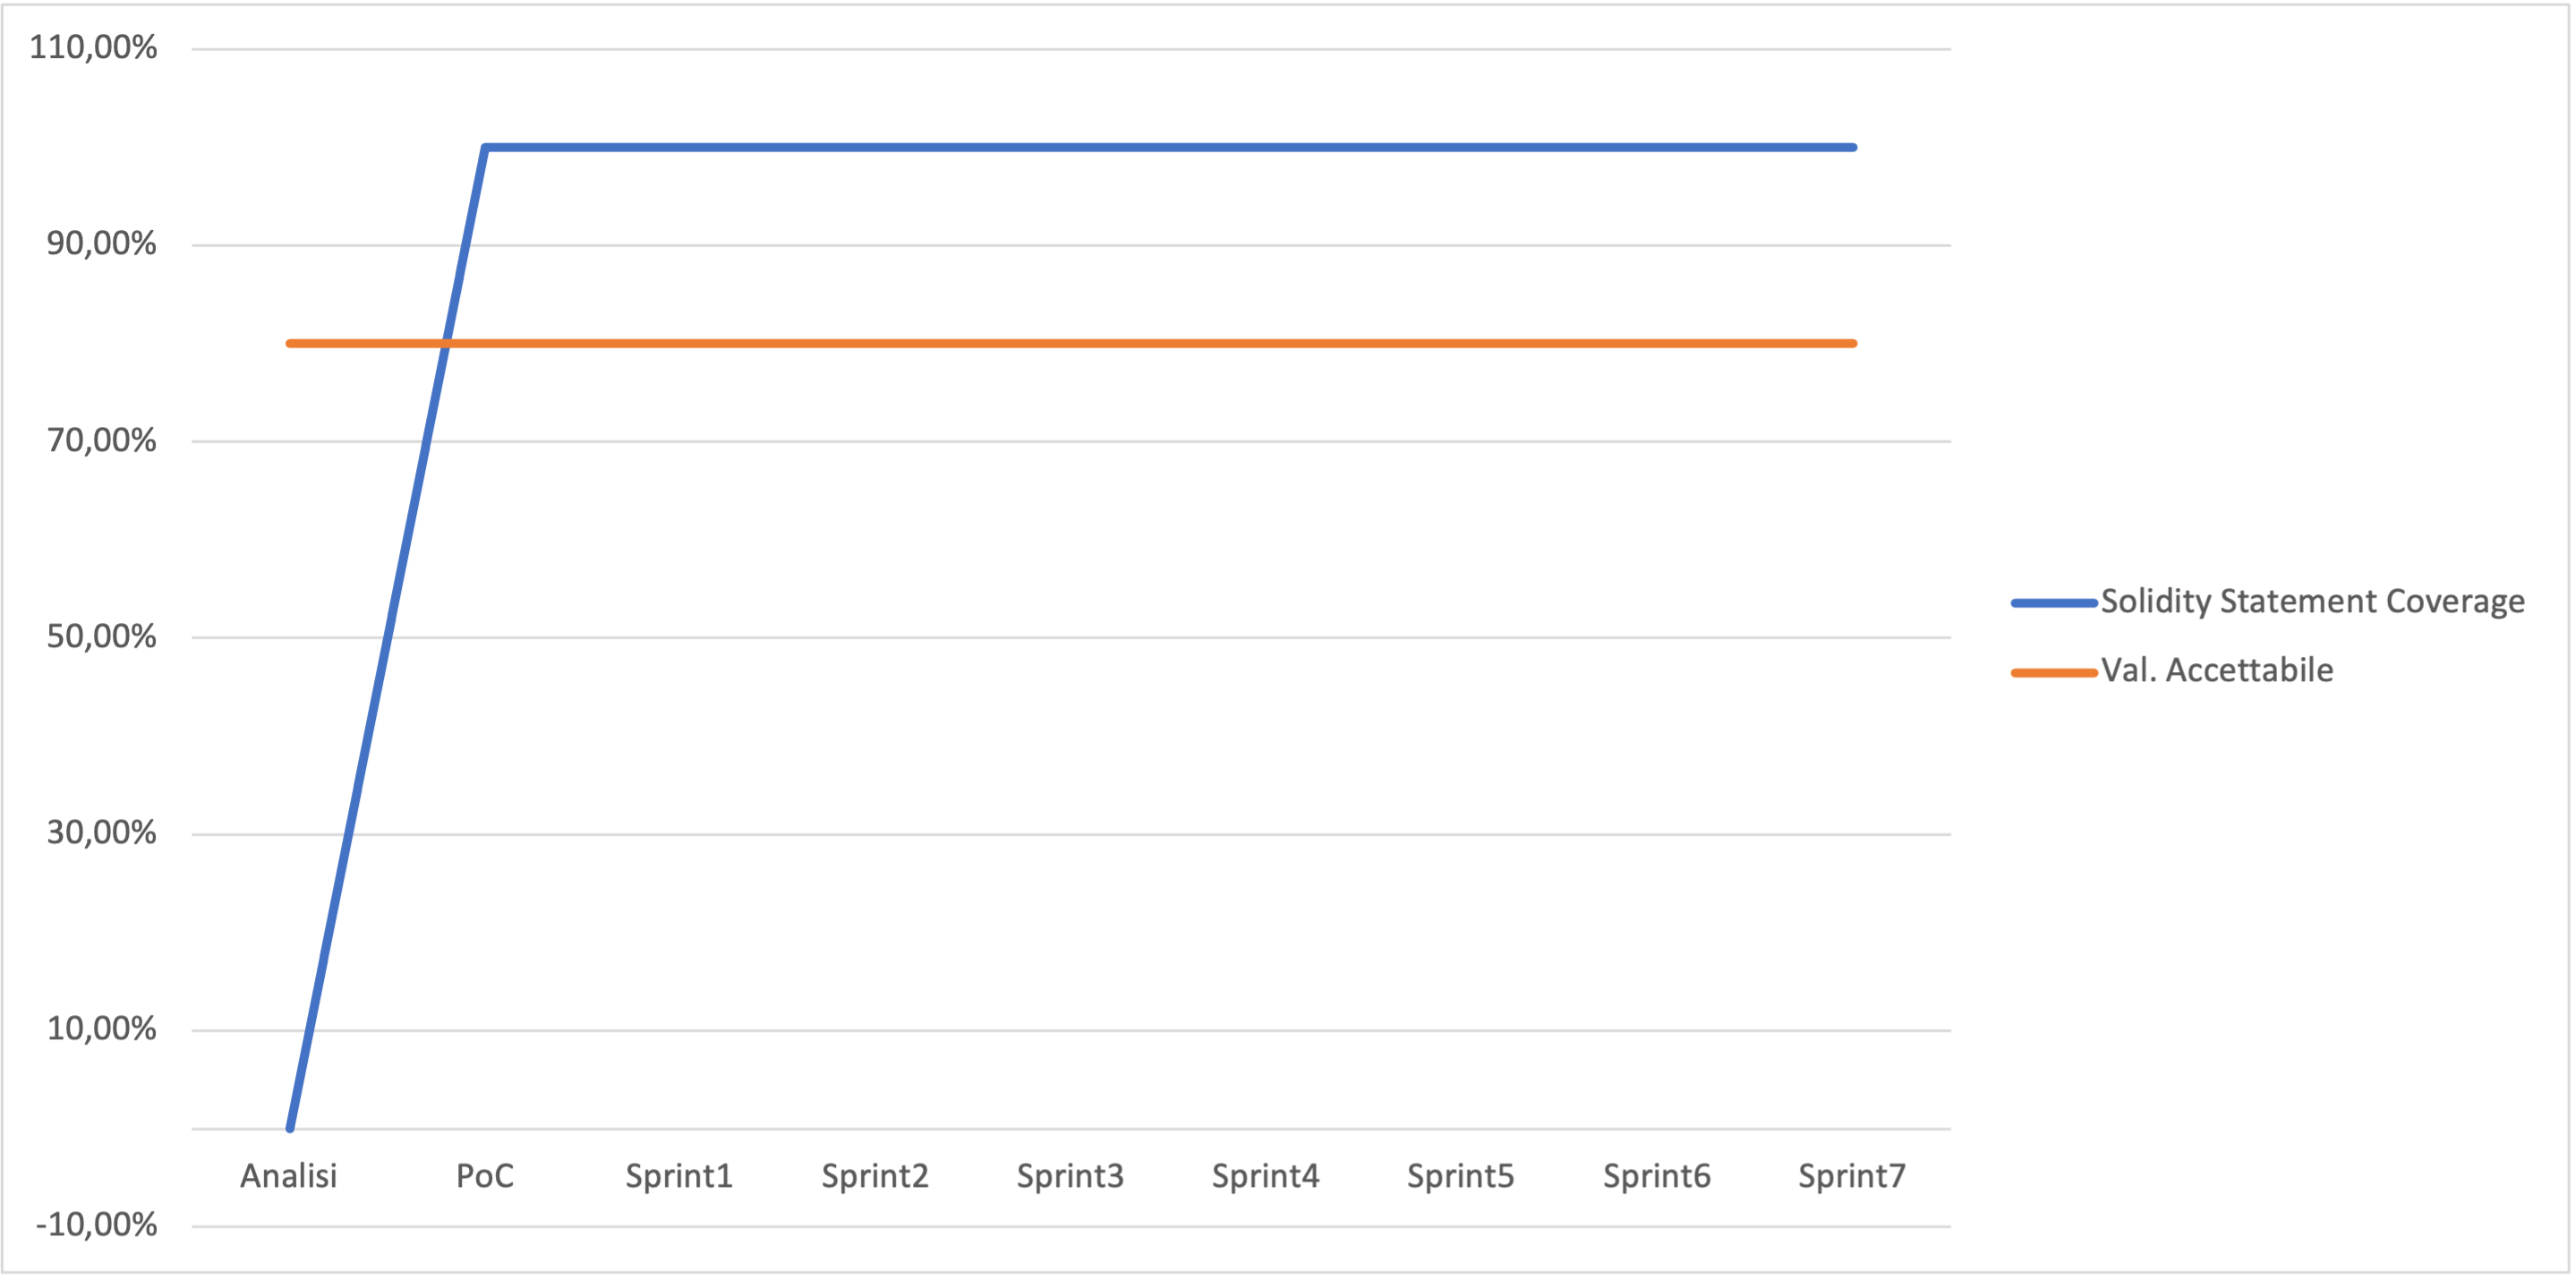
\includegraphics[width=1\textwidth]{src/img/Solidity Statement Coverage.png}
\caption{Grafico SSC}
\end{figure}

\subsubsection{Solidity Branch Coverage}

\begin{figure}[H]
\centering
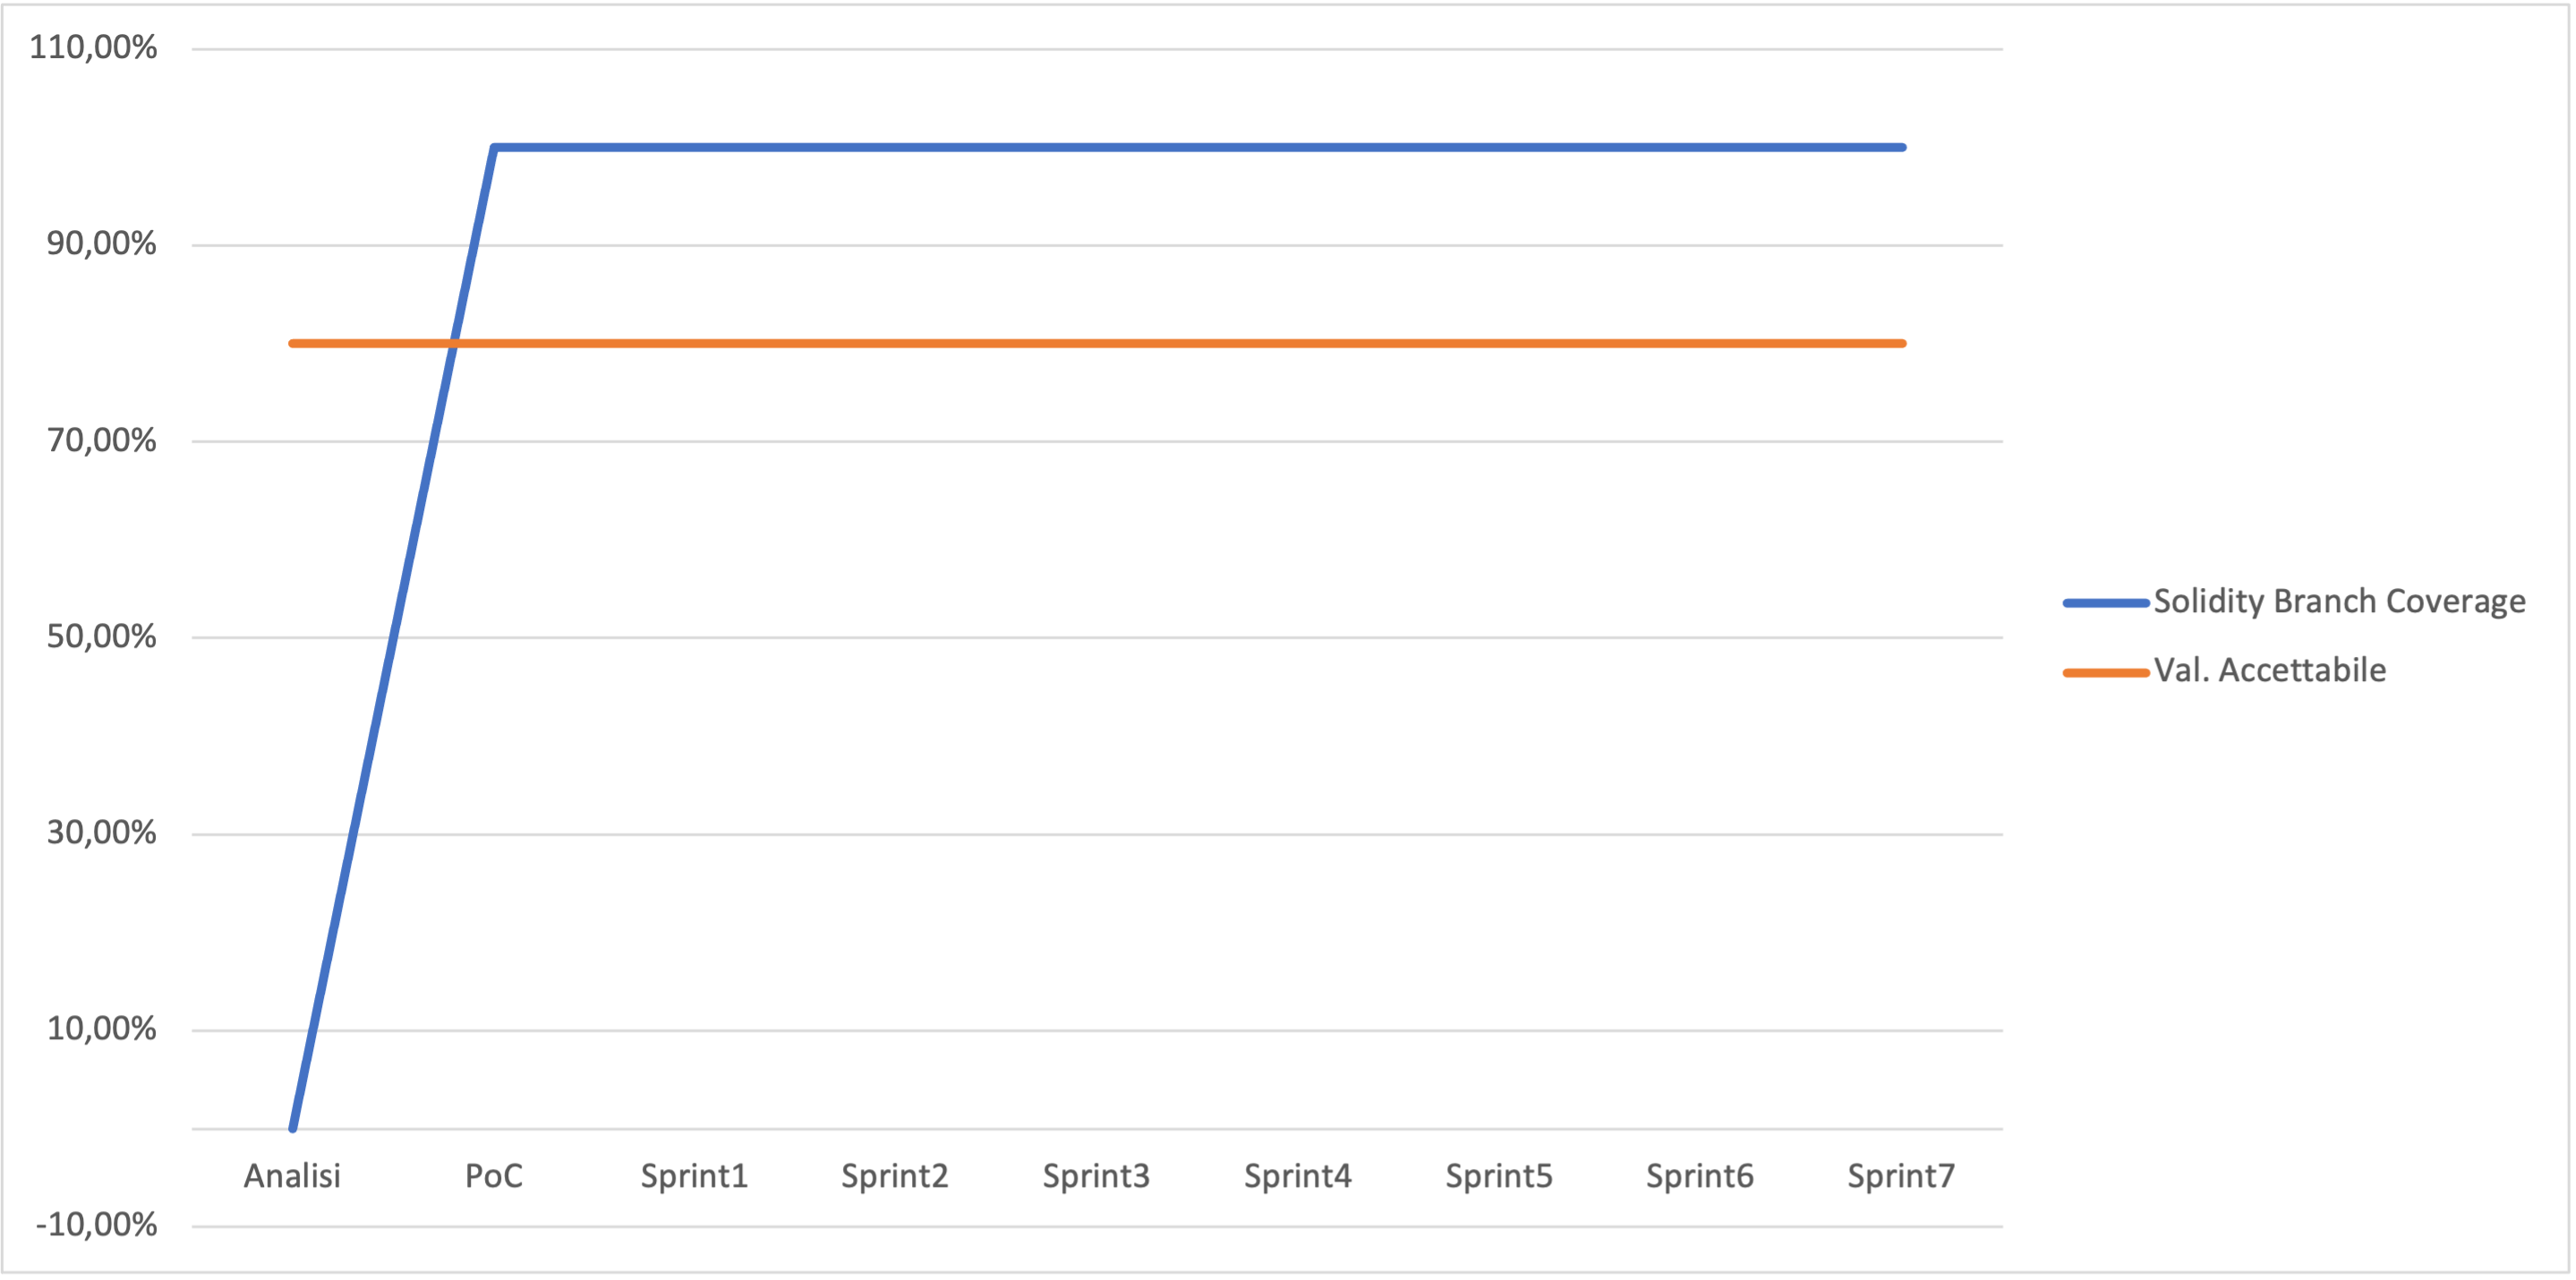
\includegraphics[width=1\textwidth]{src/img/Solidity Branch Coverage.png}
\caption{Grafico SBC}
\end{figure}

\subsubsection{Solidity Function Coverage}

\begin{figure}[H]
\centering
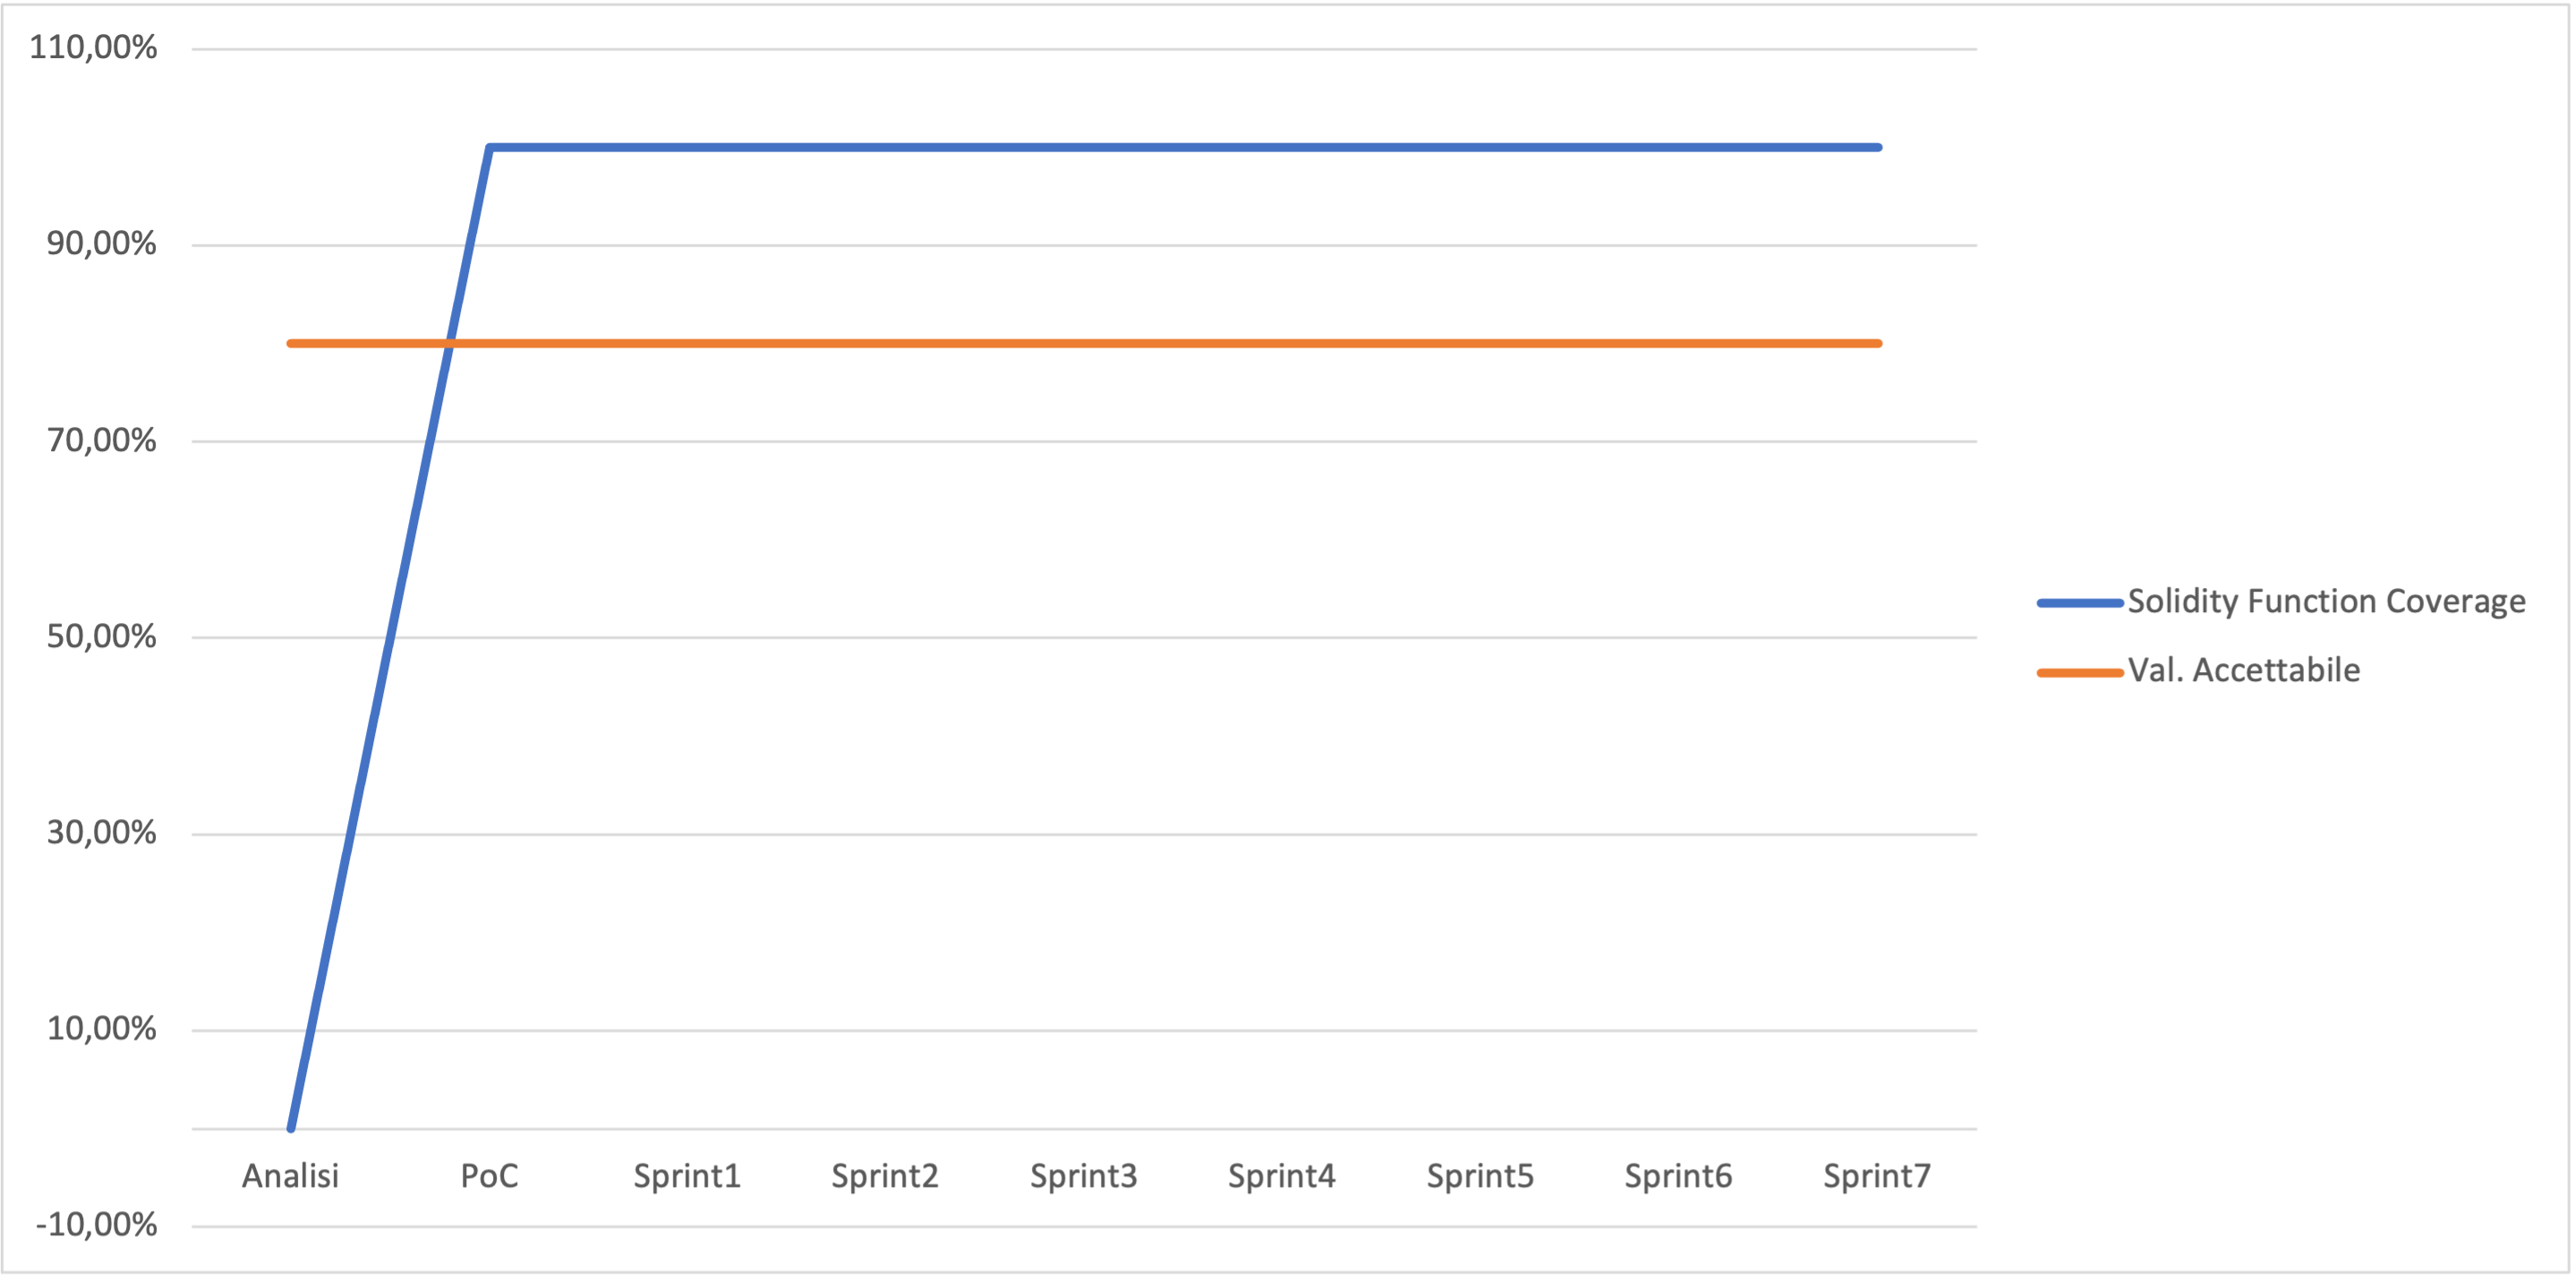
\includegraphics[width=1\textwidth]{src/img/Solidity Function Coverage.png}
\caption{Grafico SFC}
\end{figure}

\subsubsection{Solidity Line Coverage}

\begin{figure}[H]
\centering
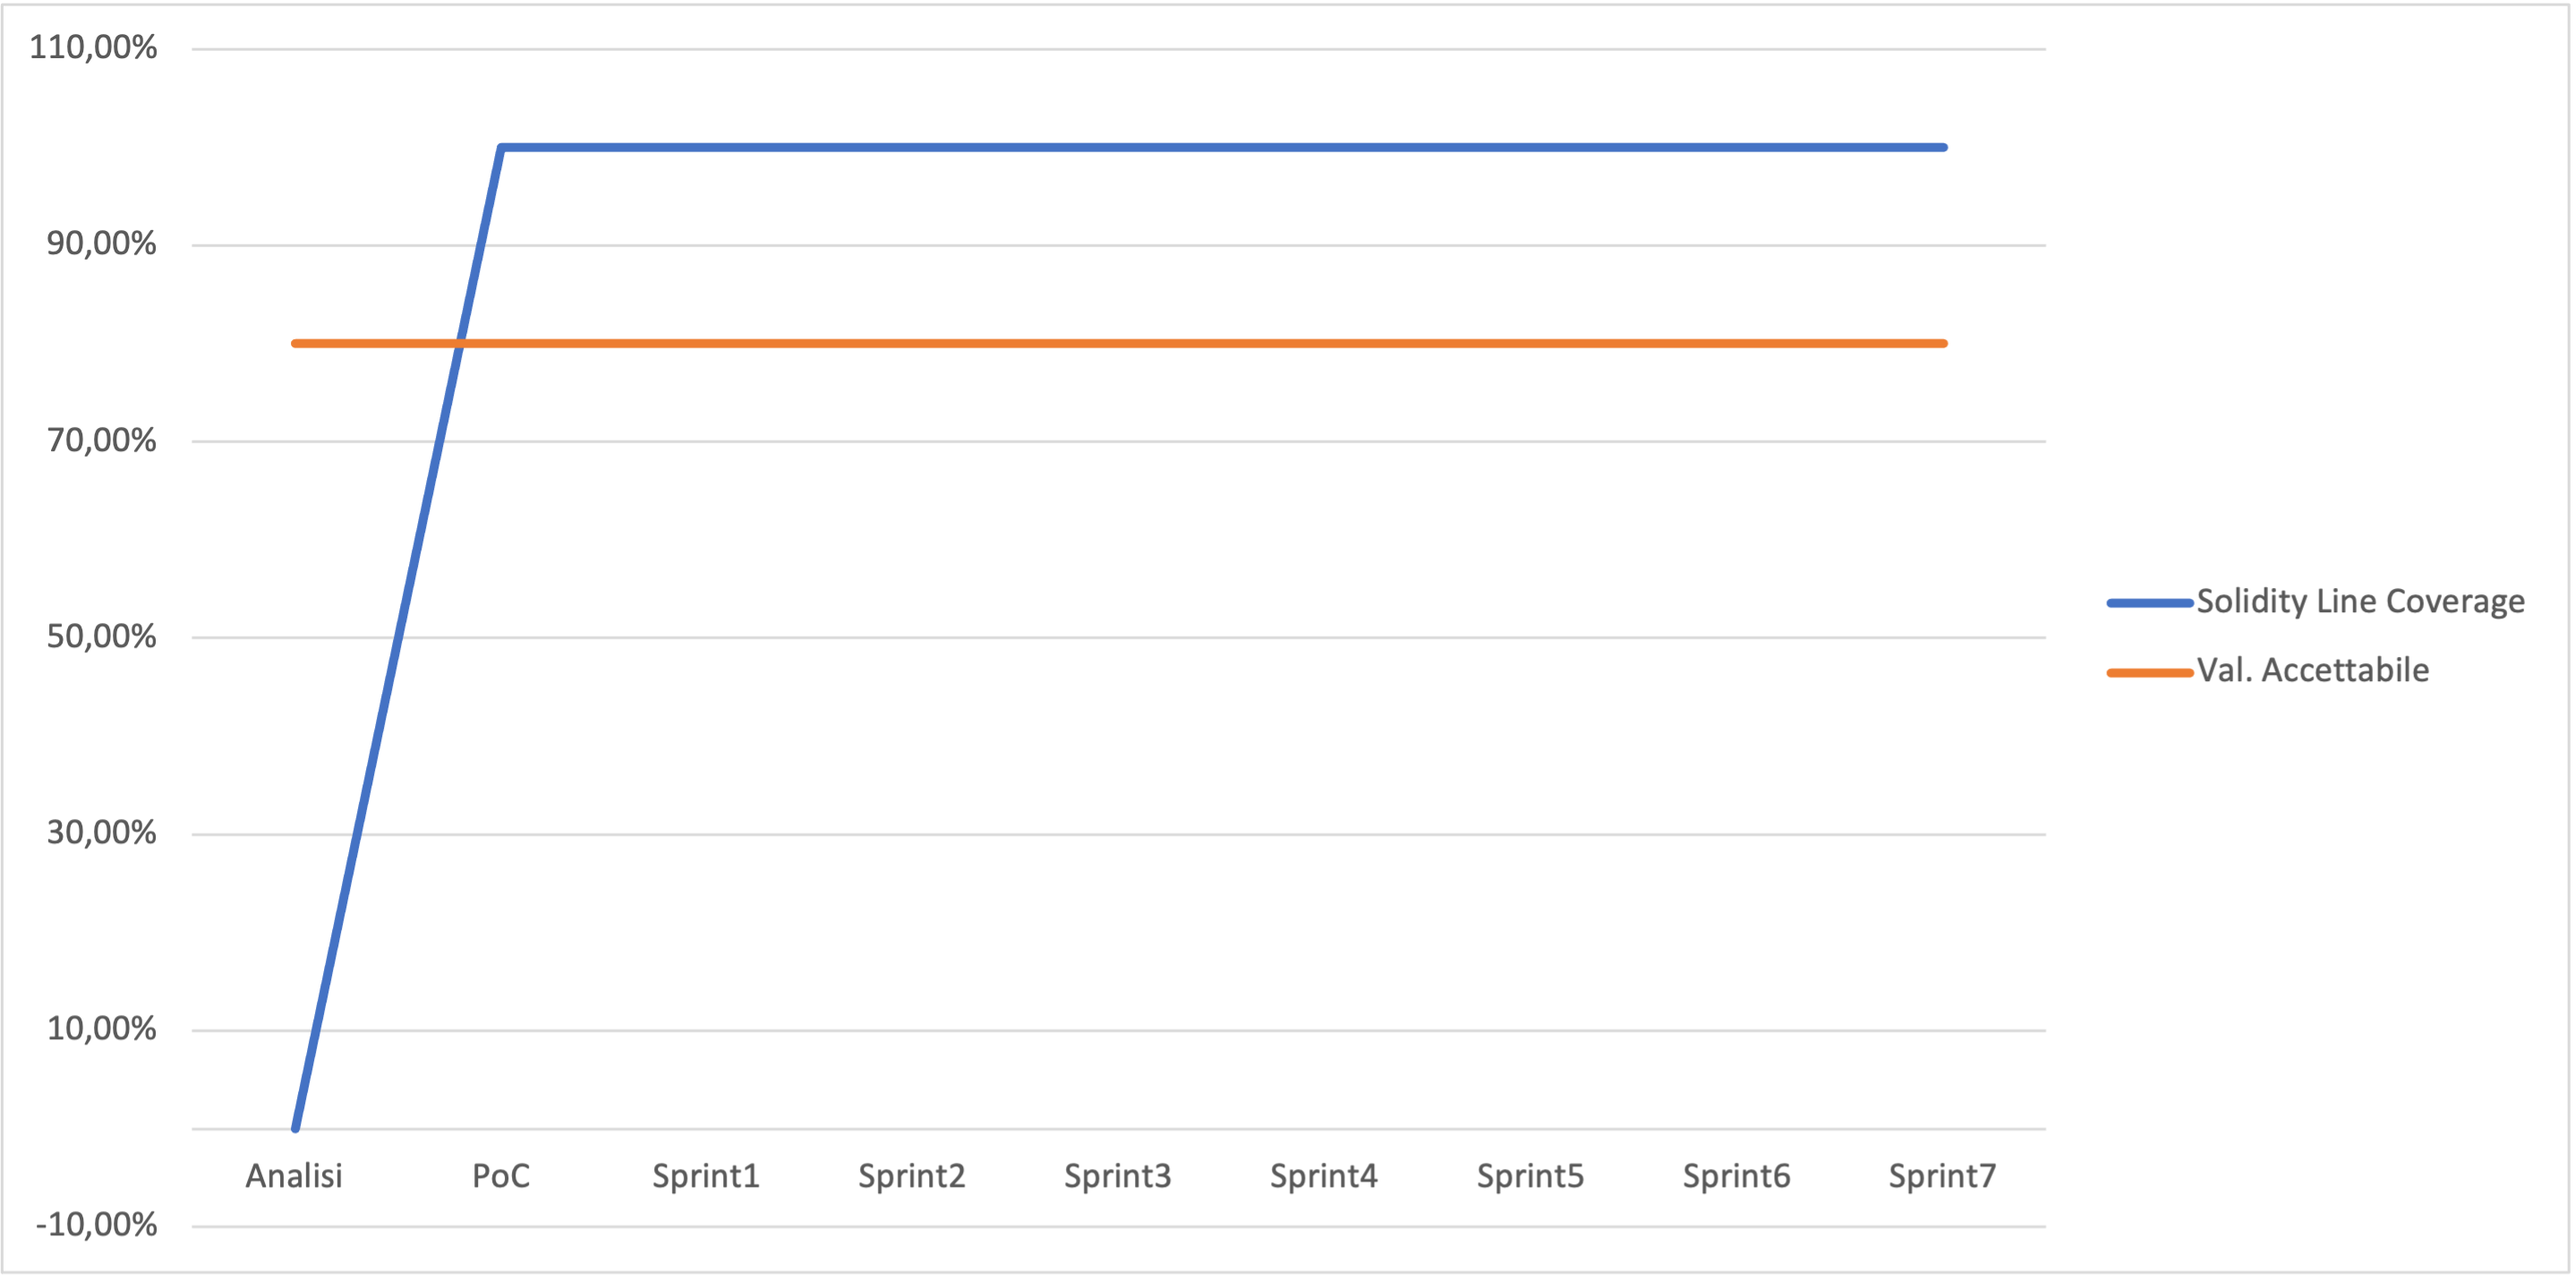
\includegraphics[width=1\textwidth]{src/img/Solidity Line Coverage.png}
\caption{Grafico SLC}
\end{figure}

\subsubsection{Frontend Statement Coverage}

\begin{figure}[H]
\centering
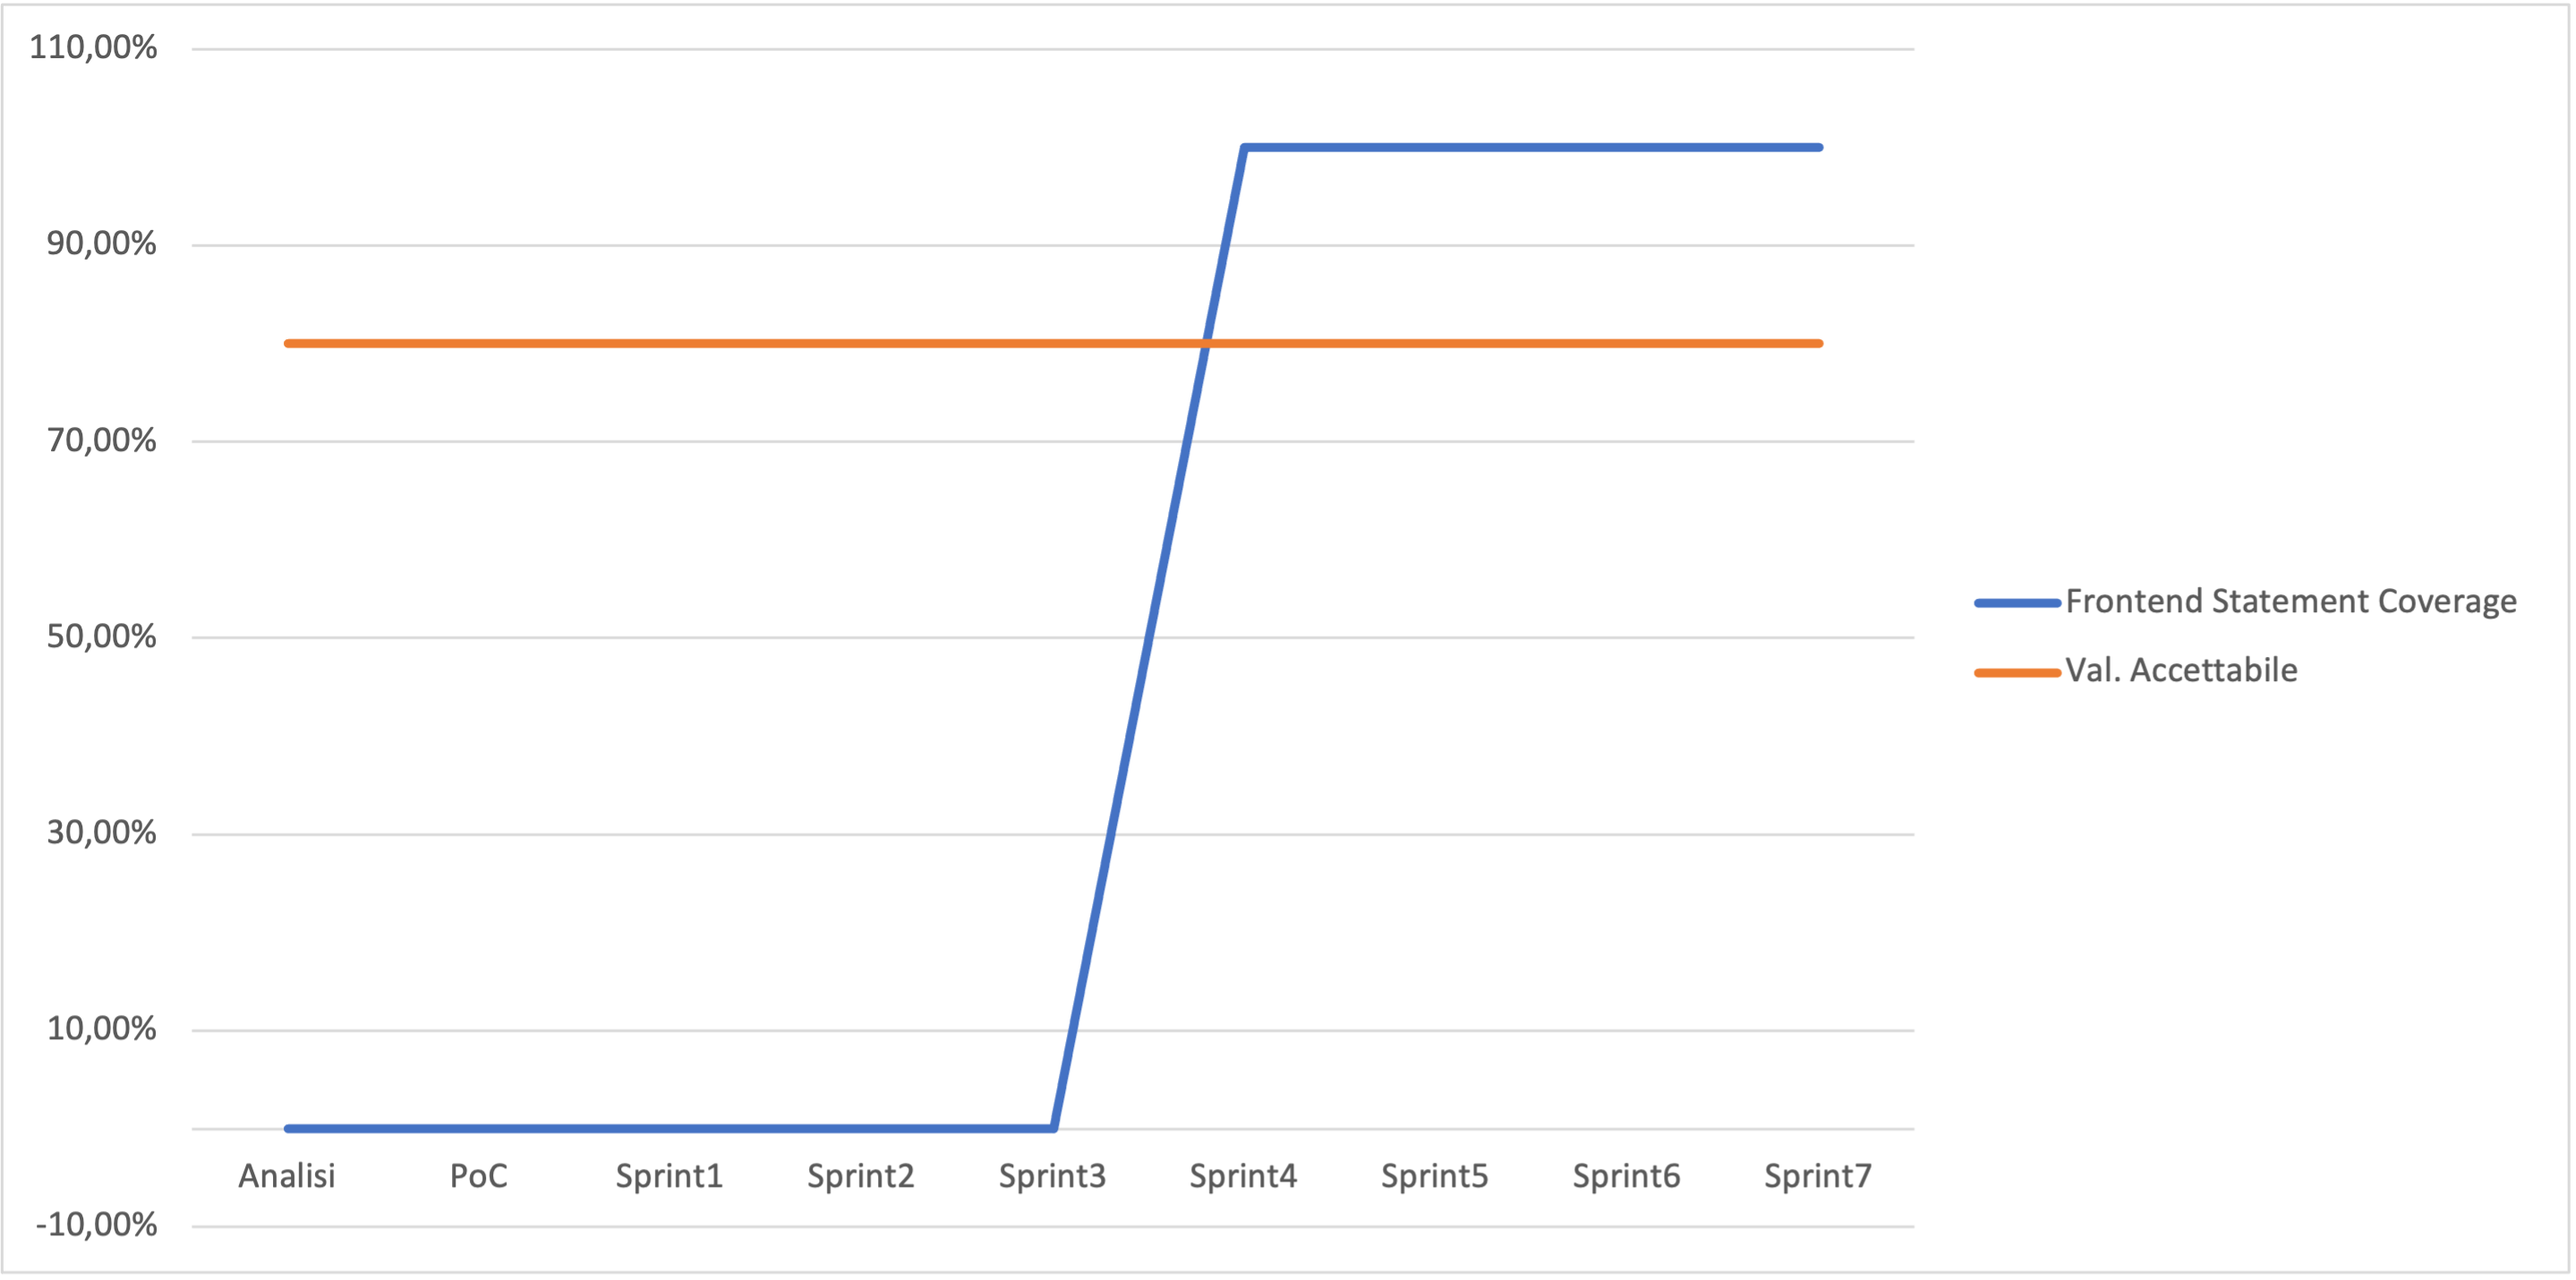
\includegraphics[width=1\textwidth]{src/img/Frontend Statement Coverage.png}
\caption{Grafico FSC}
\end{figure}

\subsubsection{Frontend Branch Coverage}

\begin{figure}[H]
\centering
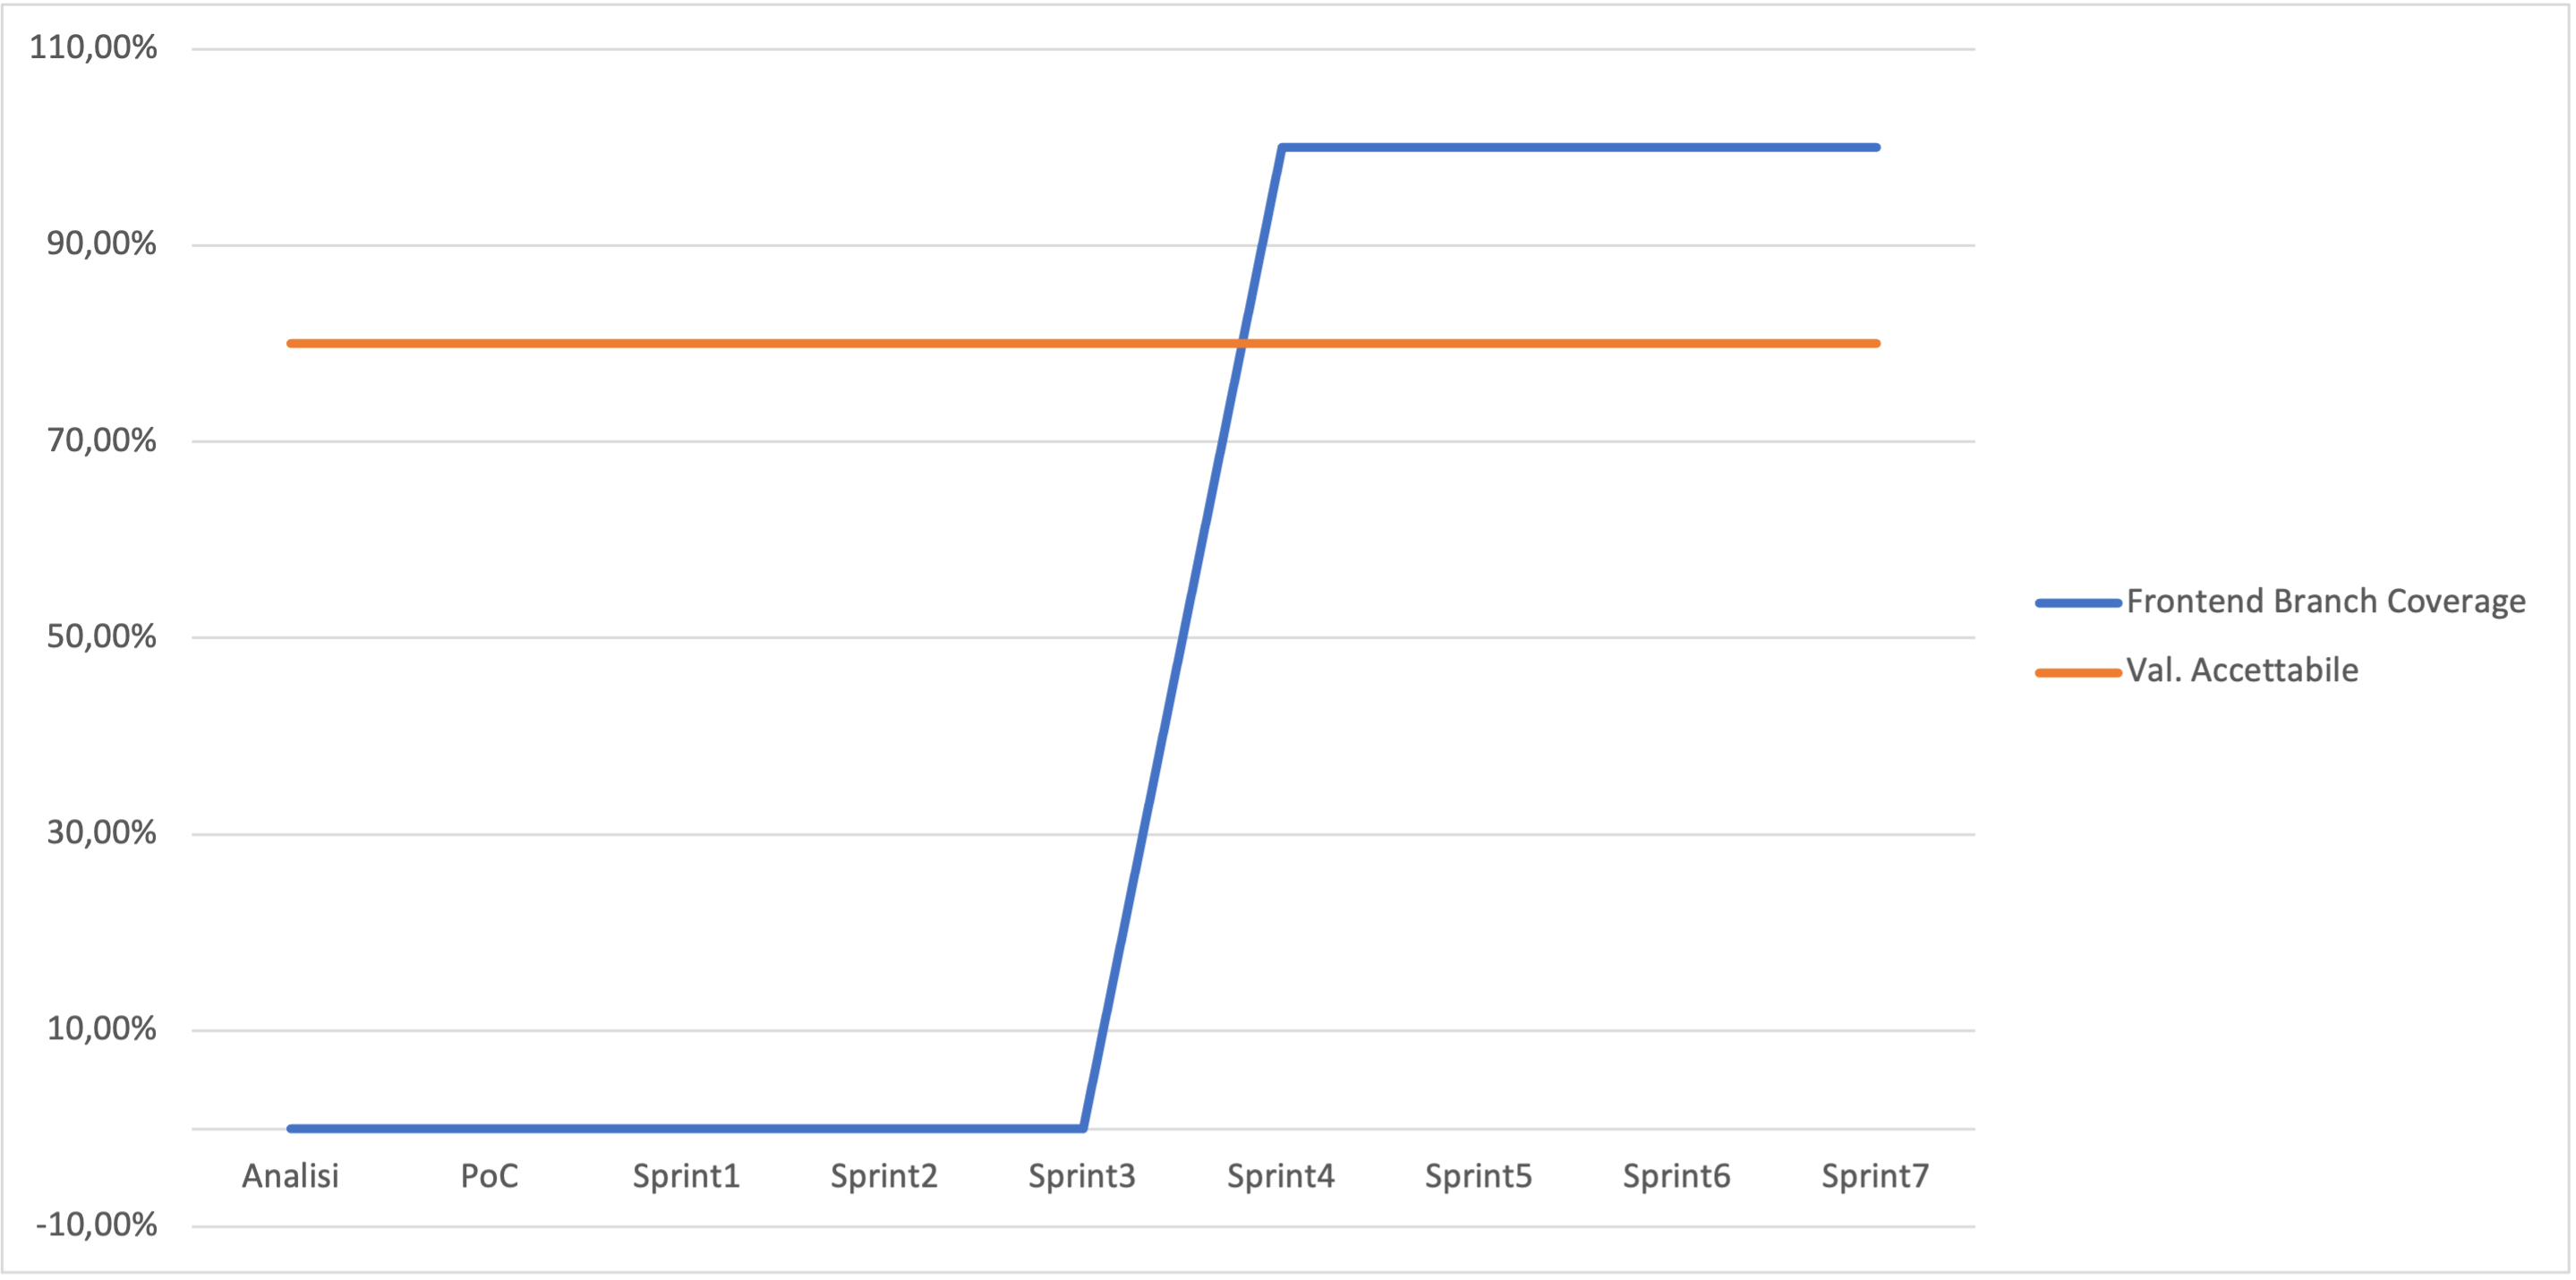
\includegraphics[width=1\textwidth]{src/img/Frontend Branch Coverage.png}
\caption{Grafico FBC}
\end{figure}

\subsubsection{Frontend Function Coverage}

\begin{figure}[H]
\centering
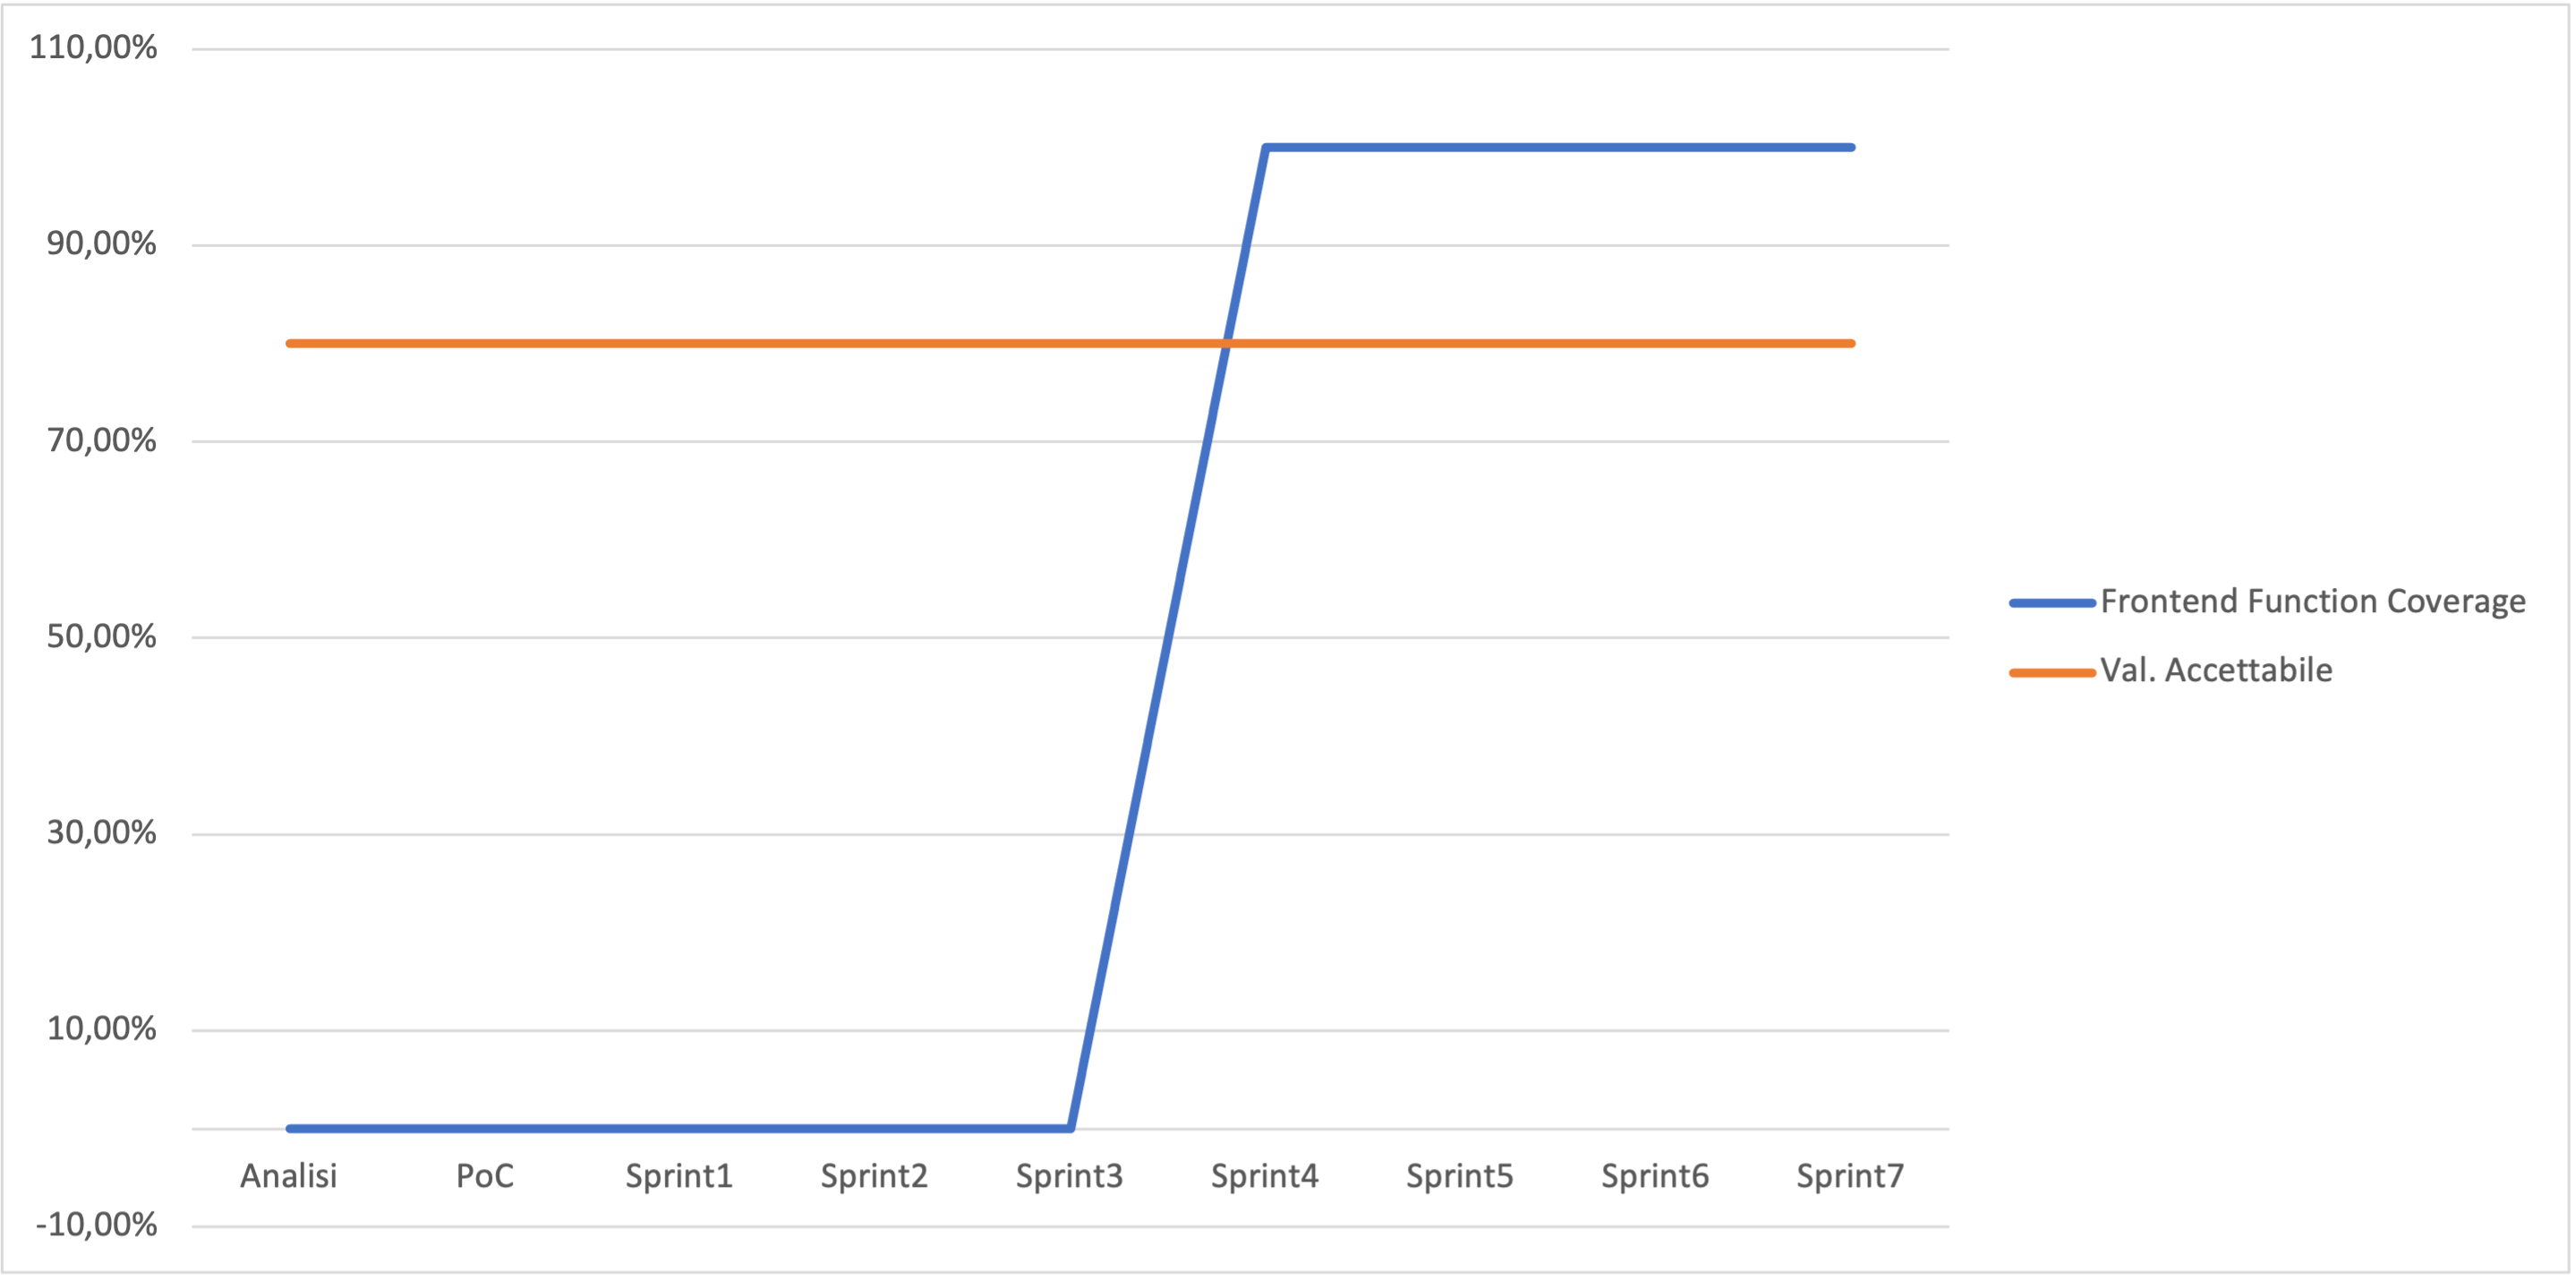
\includegraphics[width=1\textwidth]{src/img/Frontend Function Coverage.png}
\caption{Grafico FFC}
\end{figure}

\subsubsection{Frontend Line Coverage}

\begin{figure}[H]
\centering
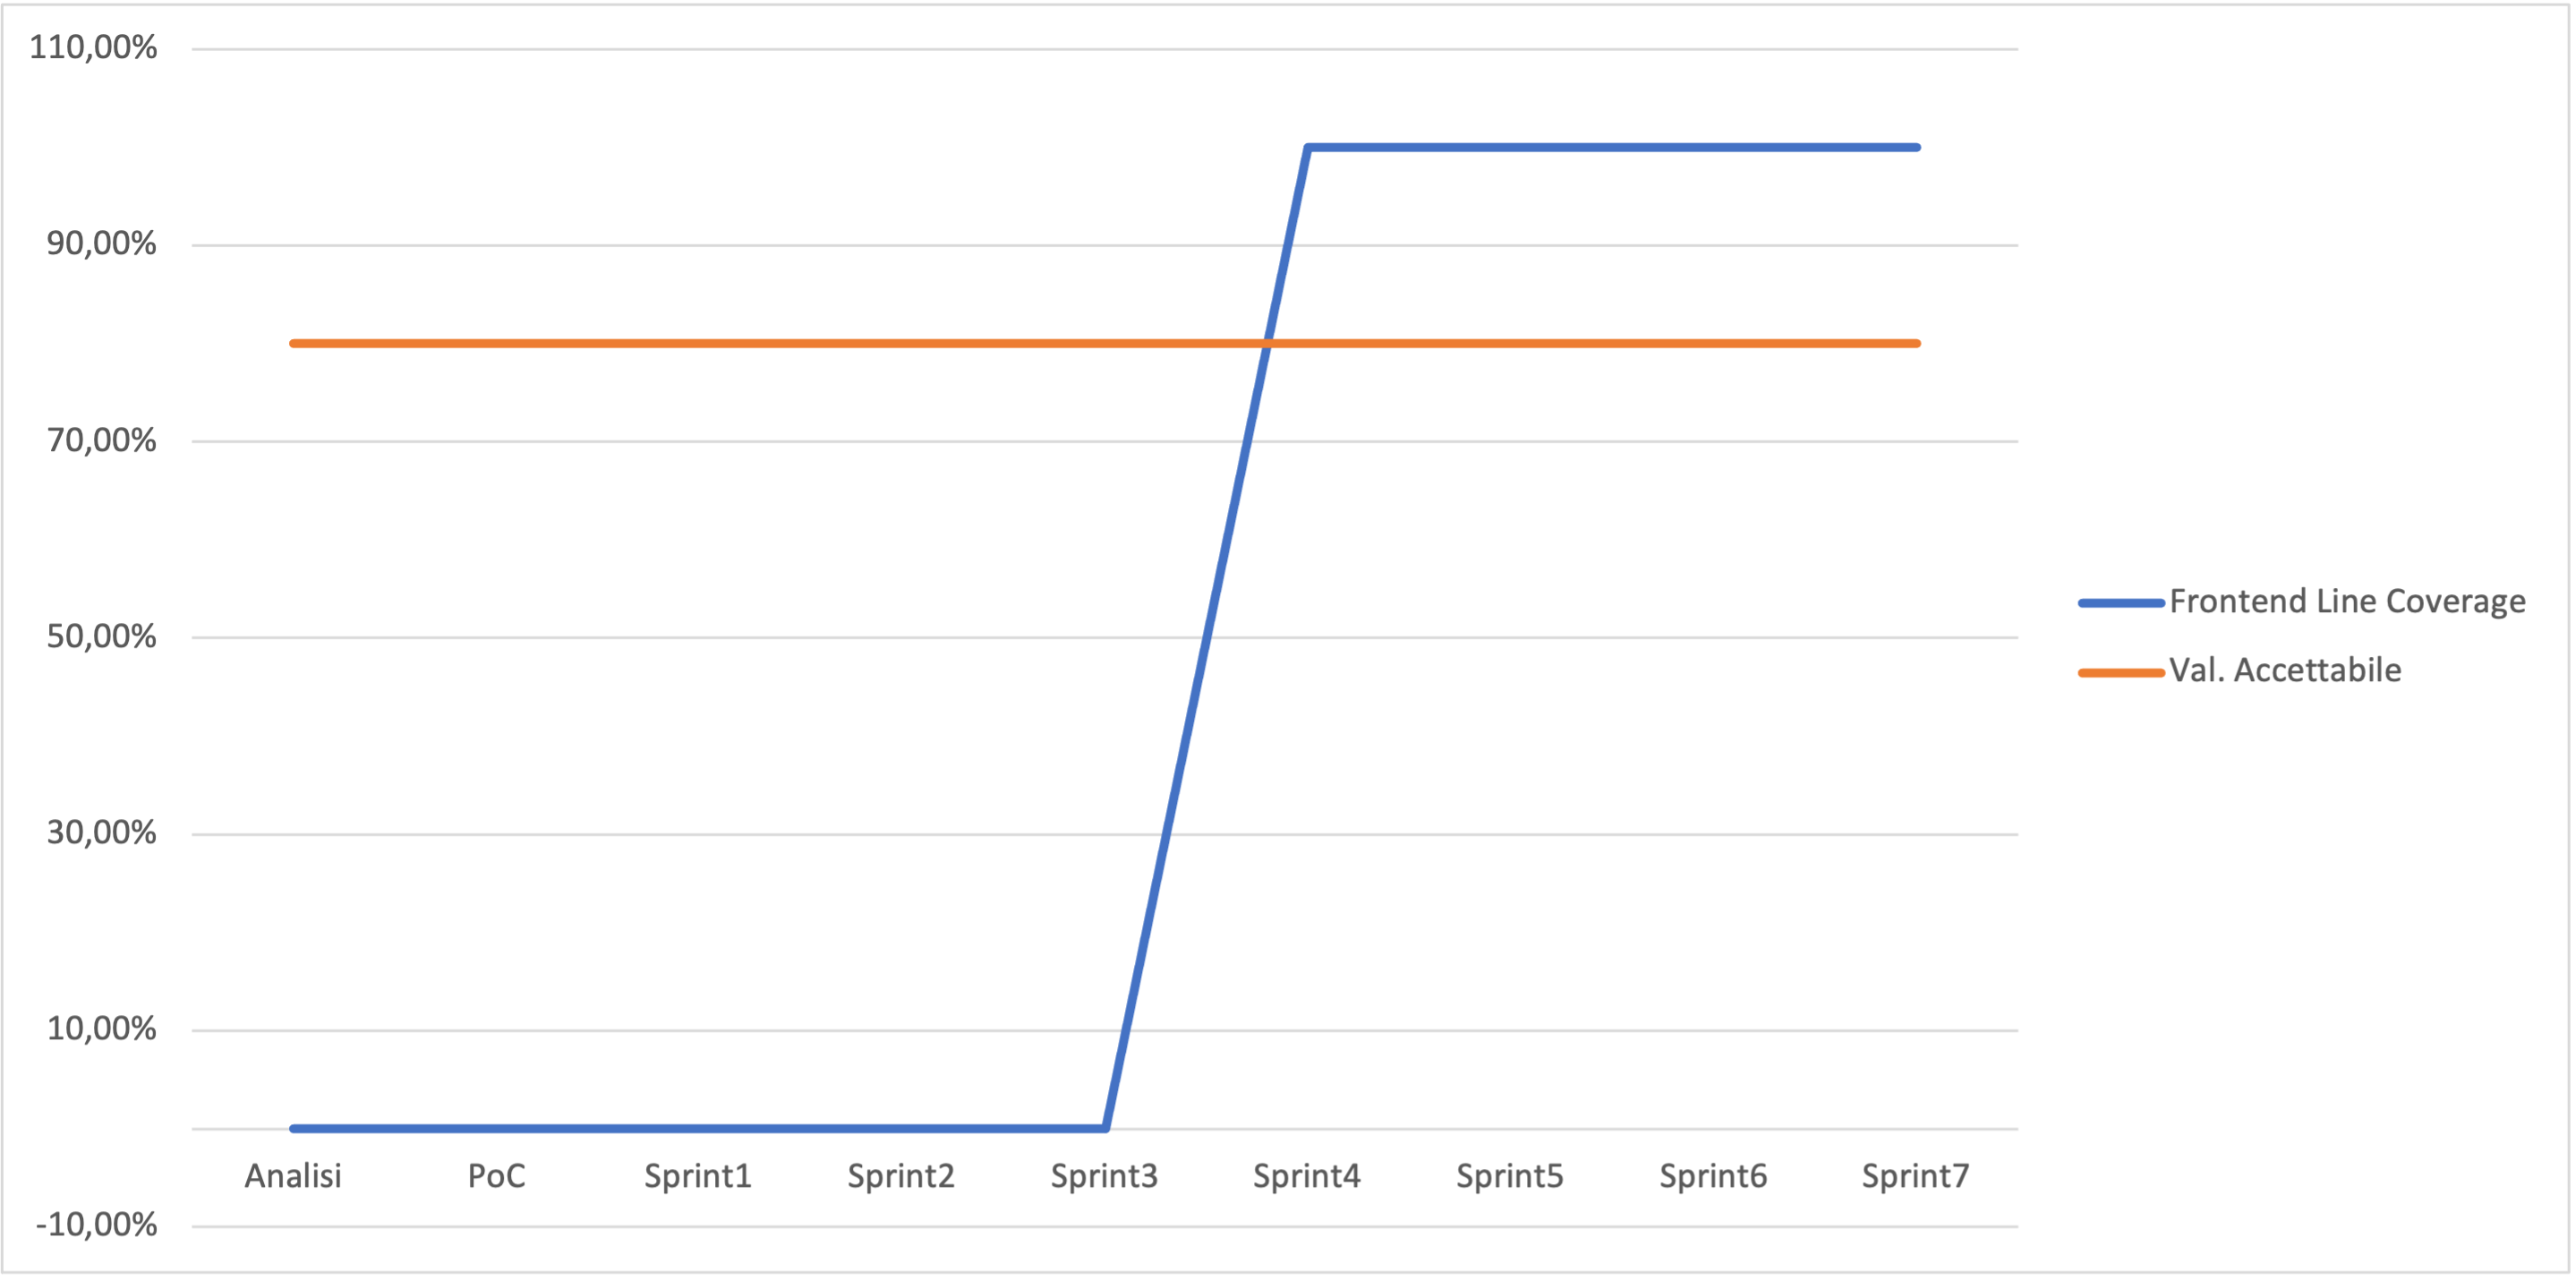
\includegraphics[width=1\textwidth]{src/img/Frontend Line Coverage.png}
\caption{Grafico FLC}
\end{figure}



















